% ============================================================================
% Asset-1 — bank paper (arXiv-grade). LaTeX conversion of
% paper/ASSET1_PAPER_DRAFT_v0.md (Director-accepted draft; wording frozen).
% House style matches paper/rhombic-xr001.tex (documentclass, package set,
% author block). Draft v0 was assembled 2026-07-21 from
% paper/asset1-sections/01-05 per ASSET1_PAPER_OUTLINE.md. Every number
% verified against docs/ASSET1_BANK_DELIVERY_2026-07-20.md (falco-root) and
% the per-item JSONs under rhombic/results/asset1-delivery-verify/; none is
% composed from memory.
% ============================================================================
\documentclass[11pt]{article}

% --- packages ---
\usepackage[margin=1in]{geometry}
\usepackage{amsmath,amssymb,amsfonts}
\usepackage{booktabs}
\usepackage{graphicx}
\usepackage{hyperref}
\usepackage{xcolor}
\usepackage{multirow}
\usepackage{float}
\usepackage[numbers]{natbib}
% \usepackage{microtype}  % disabled: MiKTeX font expansion issue (house note)
\usepackage{bookmark}

\hypersetup{
  colorlinks=true,
  linkcolor=blue!60!black,
  citecolor=blue!60!black,
  urlcolor=blue!60!black
}

% --- metadata ---
% Title: outline candidate 2, chosen because the discussion's actual
% unifying claim ("the gauge, not the information, was the obstacle") is the
% paper's mechanism, and the subtitle covers all five results. Candidate 1's
% "canonicalization is the whole story" overclaims relative to D2/D3.
\title{%
  The Gauge Is the Obstacle:\\
  Task Identity, Cross-Family Transfer, and\\
  Merge-Conflict Prediction from Adapter Weights Alone%
}

\author{%
  TASUMER MAF\\
  Timothy Bielec%
  \thanks{Corresponding author. \texttt{timothy@promptcrafted.com}}%
  , Minta Carlson
}

\date{July 2026}

\begin{document}
\maketitle

% ===================================================================
\begin{abstract}
We train a pre-registered bank of 480 LoRA adapters---2 model families
$\times$ 6 tasks $\times$ 40 seeds (Qwen2.5-1.5B-Instruct and
Llama-3.2-1B-Instruct)---and run five locked weight-only analyses against it
exactly once, under a completeness interlock, with every open analytical
choice pinned in a dated ruling before the analysis that consumed it
ran---all but one by an independent Director before the bank completed; the
exception, the D3 pair design, was declared minutes after completion, before
any pairs, merges, or labels existed, and ratified by the Director on
review. (1) Raw
adapter weights do not reveal their training task (leave-one-out accuracy
0.0792 qwen / 0.1375 llama, both failing the 1.5$\times$-chance lock at
chance 0.1667), while the $\mathrm{GL}(r)$-gauge-canonical and
vocab-signature representations identify all six tasks at 1.0000,
permutation $p = 0.000999$. (2) Our pre-registered prediction that task
structure would \emph{not} transfer across families is refuted---and refuted
specifically by the triviality control added in review: raw
transfer-at-chance was a family-scale artifact (family-identity probe 1.0000
on raw features), and shift-controlled transfer
runs 0.7375--0.7833 (binomial $p \le 1.20\times10^{-84}$). (3) The identity
backbone is the load-bearing structure: swapping trained bridges across
tasks costs less than $+0.001$ nats of validation loss; only full-entry
permutation that destroys the backbone costs $+2.8086$ (qwen) / $+3.8365$
(llama). (4) Weight-only features predict midpoint-merge conflict at
group-aware AUC 0.995 [0.983, 1.000] (qwen) / 0.962 [0.898, 0.999] (llama),
a $+0.320$ / $+0.249$ margin over a distance-only baseline with both margin
CIs excluding 0---in the weight-only, post-hoc regime, distinct from the
training-time form of merge-conflict prediction \citep{mergeprobe2026}.
(5) A pilot bridge-deviation $\leftrightarrow$ generalization-gap
correlation of $r = 0.888$ shrinks to $r = 0.300$ [0.175, 0.415] pooled at
bank scale---real, modest, and heterogeneous within task. Every headline was
independently recomputed from per-item data by the Director; Section~3.4
records the scope of each re-derivation. Two of the five
outcomes went against us, and they are the credibility of the other three;
costs and limitations are reported alongside benefits.
\end{abstract}

% ===================================================================
\section{Introduction}
\label{sec:intro}

A trained LoRA adapter is a small stack of low-rank matrices. Adapters now
accumulate by the thousands---shared on hubs, merged into products, composed
by people who never saw the training run. This paper asks what the weights
alone reveal, post hoc: given only the adapter tensors---no training data,
no logs, and no access to the training process---what can be read out, and
what does reading it out require?

The obstacle is not information but parameterization. A LoRA update
factorizes as a product of low-rank factors $BA$, and for any invertible
$r \times r$ matrix $M$ the reparameterization $(B, A) \rightarrow
(BM, M^{-1}A)$ leaves the effective update unchanged---the
$\mathrm{GL}(r)$ gauge. Two adapters trained on the same task can therefore
sit far apart in raw parameter space while encoding the same update, and two
adapters from different model families can sit apart for reasons that have
nothing to do with what they learned. Raw flattened weights are the
unexamined default of adapter analysis, and this paper measures what the
default costs.

Our answer is an artifact and a discipline. The artifact is a bank of 480
LoRA adapters---2 model families $\times$ 6 tasks $\times$ 40 seeds
(Qwen2.5-1.5B-Instruct and Llama-3.2-1B-Instruct; tasks alpaca, code, math,
xsum, squad, agnews)---trained over ${\sim}17$ days on a single local GPU.
The discipline is pre-registration with teeth: five weight-only analyses
(task identifiability within and across families, bridge-swap ablation,
merge-conflict prediction, and a pilot-correlation re-verification) were
locked before the bank completed, every open analytical choice was pinned in
a dated ruling---all but one by an independent Director before completion;
the D3 pair design was declared post-completion, before any pairs or labels
existed (Section~\ref{sec:d3design})---and a completeness interlock
refused every real-bank statistic until all 480 runs were complete. Each
analysis then ran against the real bank exactly once. Every headline number
was subsequently re-derived by the Director from per-item data---for the two
identifiability results, re-run from the feature matrices rather than from
saved predictions; for D3, his from-scratch cross-validation used the naive
fold scheme and reproduced the naive block exactly, while the group-aware
headline values were verified against the pinned report.

The results, in delivery order. First, raw adapter weights do not reveal
their training task: leave-one-out accuracy 0.0792 (qwen) and 0.1375 (llama)
against chance 0.1667, both failing the pre-registered 1.5$\times$-chance
lock---while the $\mathrm{GL}(r)$-gauge-canonical and vocabulary-signature
representations identify all six tasks at 1.0000, permutation
$p = 0.000999$. The information is in the weights; the gauge is what makes
it illegible. Second, our own pre-registered prediction that task structure
would \emph{not} transfer across model families was refuted---and refuted
specifically by the triviality control added in round-1 review. A
family-identity probe reads 1.0000 on raw representations (the families are
perfectly separable by scale), so raw transfer-at-chance was a
covariate-shift artifact; once per-family standardization removes the
family-mean separation the raw probe exploited, task
structure transfers across a 1.5B and a 1B model of different lineages at
0.7375--0.7833 (binomial $p \le 1.20\times10^{-84}$). The control converted
a would-be false confirmation into a refutation. That is pre-registration
working as designed, and we report it as the refutation it is. Third, the
trained bridge is nearly free to swap between tasks: installing a different
task's bridge costs less than $+0.001$ nats of validation loss, and only
full-entry permutation that destroys the identity backbone costs anything
($+2.8086$ qwen / $+3.8365$ llama). Fourth, two adapters' weights alone
predict whether their midpoint merge degrades, at group-aware AUC 0.995
[0.983, 1.000] (qwen) and 0.962 [0.898, 0.999] (llama)---a $+0.320$ [0.150,
0.511] and $+0.249$ [0.039, 0.490] margin over a distance-only baseline,
both margin CIs excluding 0. This is the weight-only, post-hoc regime: no
training access, distinct from the training-time form of merge-conflict
prediction (\citealp{mergeprobe2026}; Section~\ref{sec:rw}). Fifth, a pilot
correlation between bridge deviation and generalization gap ($r = 0.888$)
shrinks at bank scale to $r = 0.300$ [0.175, 0.415] pooled over 480
runs---real, positive, modest, and heterogeneous within task. We report the
shrink as a headline property of the result, not a footnote.

Two of these five outcomes---the H2 refutation and the D-aux
shrink---went against our predictions. A pipeline that
can only confirm is not a measurement instrument. The interlock, the pinned
decisions, the dated amendments, and the independent regrade exist so that
the ceiling results (H1 at 1.0000, D3 at 0.96--0.99) arrive with the same
evidentiary standing as the refutation that sits beside them.

The costs, here and in the discussion:
${\sim}17$ days of a single local GPU for the bank; two model families of
1--1.5B parameters only; 6 coarse tasks, so the label-granularity axis
(Section~\ref{sec:rw}) cuts both ways and we claim nothing about
fine-grained regimes; midpoint merges only; relative-perplexity conflict
labels;
and a distance-only baseline with a few points of fold-scheme (naive vs
group-aware) sensitivity, with the fold configuration pinned and the
fragility reported where it appears.

\paragraph{Contributions.} The bank artifact, and five results measured
against it exactly once:

\begin{enumerate}
  \item \textbf{The bank.} A 480-adapter, 2-family $\times$ 6-task $\times$
  40-seed LoRA bank, cohort-tagged and outage-audited, with a completeness
  interlock that held---no real-bank statistic was computed before
  480/480---and a per-item verification bundle from which every headline was
  independently re-derived.
  \item \textbf{The canonicalization ceiling (H1).} Raw weights fail the
  task-identifiability lock (0.0792 / 0.1375 vs chance 0.1667); the
  gauge-canonical and vocab-signature representations reach 1.0000 in both
  families. Within a controlled family, a linear probe suffices once the
  $\mathrm{GL}(r)$ gauge is removed---canonicalization, not classifier
  capacity, is the binding constraint.
  \item \textbf{The refutation-by-control (H2).} The pre-registered
  no-transfer prediction is NOT supported: raw transfer-at-chance was a
  family-scale artifact exposed by the family-identity probe (1.0000 on raw
  features; Section~\ref{sec:h2} reports the standardized probe's behavior),
  and shift-controlled transfer
  runs 0.7375--0.7833 in both directions and both representations.
  \item \textbf{The backbone result (D2).} Across 360 evaluations per
  family, every swap that preserves the identity backbone costs less than
  $+0.001$ nats; only destroying the backbone costs ($+2.8086$ /
  $+3.8365$). The backbone is the sole load-bearing structure for
  in-distribution loss.
  \item \textbf{The post-hoc merge predictor (D3).} Weight-only features
  predict midpoint-merge conflict at AUC 0.995 / 0.962 with a CI-separated
  margin over raw distance, on 120 vertex-disjoint pairs per family---the
  first supervised, held-out-evaluated conflict predictor we know of in the
  weight-only, post-hoc, no-training-access regime; weight-only conflict
  \emph{heuristics} (sign agreement, task-vector cosine) predate it
  \citep{yadav2023ties,ilharco2023task}.
  \item \textbf{The honest re-verification (D-aux).} The pilot
  deviation$\leftrightarrow$gap correlation $r = 0.888$ shrinks to 0.300
  [0.175, 0.415] at bank scale, with within-task cells shown, including a
  significantly negative one. Small-$n$, task-mixture pilot correlations do
  not survive scale, and a pre-registered bank is how you find out.
\end{enumerate}

% ===================================================================
\section{Related work}
\label{sec:rw}

\paragraph{Weight-space readout of LoRA adapters.}
Reading training provenance from full-model weights predates the LoRA era:
\citet{eilertsen2020classify} classified training hyperparameters from
weight statistics, and \citet{unterthiner2020predict} predicted accuracy
from weights alone. W2T (``W2T: LoRA Weights Already Know What They Can
Do,'' March 2026)
\citep{w2t2026lora} brought the program to LoRA scale and established that
LoRA checkpoints are legible objects:
attribute classification over collections of 10k+ adapters and retrieval
over a mixed ${\sim}$1.9k-adapter pool,
using a QR$\rightarrow$SVD canonicalization and symmetry-aware encoders that
substantially outperform raw-flattened baselines. Our regime contrast with
W2T runs on the label-granularity and task-structure axis: W2T classifies
fine-grained attribute labels (a 312-binary-attribute label space) over
collections of 10k+
adapters, where even its best models leave large headroom; we classify 6
coarse tasks, where a linear probe on canonical features reaches ceiling.
The contrast is not attributable to collection scale---W2T's collections are
themselves same-base, same-rank families (their Table 6; Stable Diffusion
vision and Llama-3.2-3B language collections)---so the
honest distinguishing variable is what the labels ask of the weights, not
how many adapters sit in the pile. Our within-family raw-vs-canonical
comparison is the complement of their result, not a contradiction of it:
both find that the raw parameterization is the obstacle, at opposite ends of
the granularity axis.

\paragraph{Canonicalization and weight-space symmetry.}
The $\mathrm{GL}(r)$ gauge is the shared enemy of this line. Learning on
LoRAs \citep{putterman2024lol} identified the $\mathrm{GL}(r)$ symmetry of
LoRA weight spaces and built equivariant processors for it; W2T's
QR$\rightarrow$SVD canonicalization is the readout-at-scale lineage our
canonical
representation follows; Spectral Geometry \citep{paul2026spectral} reads
training objective from adapter spectra with linear classifiers (AUC
$\approx 1.00$ within-method, failing cross-method); and the
symmetry-aware-encoder line W2T reports is the learned alternative to
explicit canonicalization. Our H1 result places a point on this map: within
a controlled family at coarse label granularity, no learned encoder is
needed---explicit gauge removal plus a linear SVM is already at ceiling, and
the same features left in the raw gauge fail a 1.5$\times$-chance lock.
Canonicalization is the whole story at this operating point.

\paragraph{Merge-conflict prediction.}
arXiv:2606.19549 \citep{mergeprobe2026} (June 2026) owns the training-time
form of this problem: predicting merge conflict with access to the training
process. Our D3 result is scoped exactly as our experiment card scoped
it---weight-only and post-hoc, from the two adapters' tensors alone, with no
training access---and we claim only that regime. Their MERGE-PEFT benchmark
(introduced in the same work) is the shared evaluation territory both forms
will eventually meet on. The two regimes answer different operational
questions: theirs, whether a conflict can be anticipated while training is
still running; ours, whether a repository of finished adapters can be
triaged for mergeability with nothing but the files. The quantity D3
predicts---whether the $\alpha = 0.5$ midpoint interpolation degrades
endpoint loss---is the loss barrier of the linear-mode-connectivity
literature \citep{frankle2020lmc,entezari2022perm}, and Git Re-Basin
\citep{ainsworth2023rebasin} removes permutation barriers between full
networks; D3 asks the supervised, weight-only version of that question for
LoRA updates. Weight-only conflict heuristics---sign agreement in
TIES-merging \citep{yadav2023ties} and task-vector geometry
\citep{ilharco2023task}---predate our predictor; D3's contribution is the
supervised, held-out-evaluated form.

\paragraph{Weight-only diagnostics in kind.}
Reading properties of a model from its weights alone has precedent outside
merge prediction: backdoor forensics from adapter weights
\citep{backdoor2026}, interpretation of customized-model weight spaces
\citep{w2w2024}, and WeightWatcher's
PEFT mode (Martin \& Mahoney's spectral tool applied to the $BA$ delta
matrices) \citep{martinmahoney_weightwatcher,martin2024wwpeft}, whose
overfit-adjacent diagnostics---the peer-reviewed line runs through
\citet{martinmahoney2021nature}, and the predicting-generalization program
through \citet{jiang2020fantastic}---are the neighborhood our D-aux
re-verification
lives in. Our contribution to this kind is less any single detector than the
evidentiary standard: a pre-registered bank large enough to shrink a pilot
correlation honestly.

\paragraph{Method provenance.}
The operational method that produced these numbers---typed state blocks over
prose restatement, maker--grader separation, pre-registration with pinned
decisions and dated amendments---is the house discipline measured in
rhombic-xr001 \citep{bielec2026typedstate} and enforced here by the
experiment card and Director-decision protocol. We cite it for method
provenance, not for numbers; no result from that work enters this paper.

% Citation verification pass (2026-07-21, fresh-context agent, R4):
% all four arXiv IDs fetched and VERIFIED against abstracts/full text ---
% 2603.15990 (W2T, title verbatim), 2604.08844 (Spectral Geometry; note
% n=38, one family), 2606.19549 (MergeProbe/MERGE-PEFT; training-time
% scoping confirmed at all six citation sites), 2602.15195 (backdoor
% forensics, 600/family benchmark). Three wording fixes applied in this
% pass: 10k+ = ADAPTER count not class count (classes <= 312) at three
% sites; MERGE-PEFT re-attributed to 2606.19549 itself; "WeightWatcher-
% PEFT" -> WeightWatcher PEFT mode (Martin & Mahoney) + blog citation.
% Remaining for the LaTeX pass: full BibTeX entries incl. the
% WeightWatcher tool/blog reference.

% ===================================================================
\section{Experimental design and methods}
\label{sec:design}

\subsection{The adapter bank}
\label{sec:bank}

The artifact under study is a bank of 480 LoRA adapters: 2 model families
$\times$ 6 tasks $\times$ 40 seeds. The families are Qwen2.5-1.5B-Instruct
and Llama-3.2-1B-Instruct; the tasks are alpaca, code, math, xsum, squad,
and agnews. Every run trains a rank-24 adapter on the q/k/v/o projections,
with a 6-channel identity-initialized bridge per wrapped module: the rank-24
intermediate activation is reshaped into 6 channels of 4, a learnable
$6 \times 6$ matrix $M$ mixes the channels, and the result is reshaped
back---so the effective update is $\Delta W = B\,(M \otimes I_4)\,A$, the
bridge acts on the rank space as the block matrix $M \otimes I_4$, and its
36 learnable entries are the positions that Section~\ref{sec:d2}'s
permutation cells operate on. At identity initialization the bridge is
exactly absent ($\Delta W = BA$, standard LoRA); this is the house
architecture whose trained structure D2 and D-aux measure. Training uses
plain
language-modeling loss on all tokens: sequences are padded to a fixed length
of 512 with \texttt{labels = input\_ids.clone()} and no $-100$ masking, so
every sequence contributes 511 equally weighted shifted token losses. Each
run takes 2000 optimizer steps at effective batch 16 (micro-batch 4 $\times$
gradient accumulation 4), consuming 32,000 training sequences from a
per-task pool capped at 40,000 examples. The pool is reshuffled each epoch,
deterministically in the run's data seed; pools smaller than the demand
cycle through multiple epochs (the math pool cycles ${\sim}4.6$ epochs), so
every run's data order is a pure function of its seeds. Training seeds
derive from \texttt{seed\_base = 10000} and \texttt{data\_seed\_base =
20000} by run index. Validation is a fixed 500-example split per task, cut
with the locked \texttt{val\_seed = 777}---the same split for every analysis
that touches val loss. Adapter module counts are discovered from each
adapter rather than hardcoded: 112 modules per run for Qwen, 64 for Llama.

The batch geometry deserves one paragraph, because it changed mid-campaign
under a dated amendment (A1, Director-adopted 2026-07-06). The original
geometry was micro-batch 2 $\times$ accumulation 8; the amendment moved to
4 $\times$ 4 with the effective batch unchanged, after verifying the three
conditions for bit-equivalence up to float summation order: the models use
RMSNorm (no batch normalization) and the adapters are linear; the gradient
clip fires once per optimizer step on the accumulated gradient; and the LR
schedule counts optimizer steps, so both geometries see identical sequences
over identical steps. All 480 runs were re-executed at 4 $\times$ 4 for
provenance uniformity, not correctness, and every config records its batch
geometry as a cohort tag so cohorts are never silently mixed.

The campaign ran on a single local GPU from July 3 21:52Z to July 20
16:21Z---roughly 17 days including the A1 restart, at about 1.9$\times$ the
original throughput. The manifest closed at 480/480 COMPLETE on
2026-07-20T16:21:19Z. The outage ledger contains exactly four failures, all
HF Hub 504 errors on July 16 (run indices 329--332), all retried to
COMPLETE. One run-log item from the analysis phase belongs in the open: the
first D1 launch died on a default-HF-cache environment trap and was
relaunched clean---an environment-level failure that unblinded nothing.
Chance accuracy for the 6-task classification problems throughout is 0.1667.

Table~
ef{tab:t1-bank-design} collects the full design and training
configuration, generated from the bank manifest and trainer source rather
than transcribed; Table~
ef{tab:t2-datasets} identifies the task sources
and formatting.

% AUTO-GENERATED by make_t1.py from asset1_bank.py + asset1_datasets.py +
% bank_manifest.json — regenerate, never hand-edit values.
\begin{table}[t]
\centering
\small
\begin{tabular}{@{}p{0.32\linewidth}p{0.62\linewidth}@{}}
\toprule
\textbf{Design element} & \textbf{Value} \\
\midrule
Bank shape & 2 families $\times$ 6 tasks $\times$ 40 replicates = 480 runs (all COMPLETE) \\
Families & Qwen2.5-1.5B-Instruct / Llama-3.2-1B-Instruct \\
Tasks & alpaca, code, math, xsum, squad, agnews \\
LoRA rank / alpha / channels / bridge & r=24, $\alpha$=16.0, 6 channels, identity-initialized bridge \\
Target modules & \texttt{q\_proj}, \texttt{k\_proj}, \texttt{v\_proj}, \texttt{o\_proj} \\
Optimizer & AdamW (lr, weight decay explicit; \(\beta\), \(\epsilon\) library defaults) \\
Peak LR / weight decay / clip & 0.0002 / 0.01 / max-norm 1.0 \\
LR schedule / warmup & linear warmup then cosine decay to a 0.1 floor; 100 warmup steps \\
Steps / batch geometry & 2000 optimizer steps $\times$ (batch 4 $\times$ accum 4) = effective 16; 32,000 sequences \\
Sequence length & 512 tokens \\
Precision & bfloat16 base model; float32 adapter parameters \\
Loss & LM loss over the full padded sequence (labels = input ids; no prompt/pad masking) \\
Seeds & train 10000+run\_index; data 20000+run\_index; val split seed 777 \\
Pools / validation & pool cap 40,000 per task; fixed 500-example val split per task (seed 777, identical across runs) \\
Eval cadence & train+val loss every 100 optimizer steps \\
\bottomrule
\end{tabular}
\caption{Asset-1 bank design and training configuration. Every run
records its full config and library versions in its own
\texttt{config.json}; the bank manifest pins per-run seeds and status.}
\label{tab:t1-bank-design}
\end{table}

% AUTO-GENERATED by make_t1.py — dataset identities (dossier item C).
\begin{table}[t]
\centering
\small
\begin{tabular}{@{}llp{0.5\linewidth}@{}}
\toprule
\textbf{Task} & \textbf{Source dataset (HF id)} & \textbf{Formatting} \\
\midrule
alpaca & \texttt{yahma/alpaca-cleaned} & instruction(+input) $\to$ response, Alpaca-style \#\#\# template \\
code & \texttt{sahil2801/CodeAlpaca-20k} & instruction(+input) $\to$ response, same template family \\
math & \texttt{openai/gsm8k (config main)} & step-by-step solve instruction; question $\to$ answer \\
xsum & \texttt{EdinburghNLP/xsum} & summarize instruction; document (token-budget truncated) $\to$ summary \\
squad & \texttt{rajpurkar/squad (v1.1)} & answer-from-passage instruction; context+question $\to$ first gold answer \\
agnews & \texttt{fancyzhx/ag\_news} & 4-way classify instruction; text $\to$ class name \\
\bottomrule
\end{tabular}
\caption{Task sources. All six load the HF \texttt{train} split; a single canonical shuffle (seed 777) fixes a 500-example validation split and a 40,000-example training pool per task; per-run order is reshuffled by \texttt{data\_seed}.}
\label{tab:t2-datasets}
\end{table}


\subsection{Pre-registration machinery}
\label{sec:prereg}

The analyses were pre-registered in three layers, each with a paper trail.

\paragraph{The locked experiment card.} The hypotheses (H1, H2, H3, the D3
prediction target, the D-aux re-verification) were locked in the experiment
card of 2026-07-03, before the bank existed. The card's standing instruction
is that hypotheses are locked and the deliverable fills result tables only.
One provenance gap is reported rather than papered over: the card was
maintained outside version control during the campaign and enters the
repository only with this paper
(\texttt{docs/asset1\_experiment\_card\_2026-07-03.md}, committed
retroactively); its date is the document's own, corroborated by the
2026-07-06 pipeline documentation that cites it.

\paragraph{Director-pinned decisions.} The Director is a separate AI
reviewer instance with no shared context with the authors (see
Acknowledgments) and no role in authoring the
analyses; ``pinned'' means committed in a dated ruling before the consuming
analysis ran, and ``locked'' means a pre-registered pass criterion. Every
analytical choice the card left
open was pinned by the Director on 2026-07-06---before the bank
completed---and baked into the analysis tools, which record each pinned
choice in their output JSON so runs self-document. The pins that carry the
results in this paper: the H2 decision rule (one-sided exact-binomial
$\alpha = 0.01$ and a $\ge 15$ percentage-point within-minus-cross margin,
required in \textbf{both} transfer directions, evaluated on the
shift-controlled representation with raw reported as descriptive); the D2
structure reference (\texttt{permuted\_deviation} is the primary H3
reference, with the full-entry permutation retained as the identity-backbone
contrast) and the ruling that the magnitude/topology decomposition cells run
unconditionally, because gating them on whether a contradiction materializes
would be a post-hoc forking point; and the D3 label rule (a fixed 5\%
relative-degradation threshold per endpoint, with a degenerate floor at
10\% class balance below which the analysis falls back to a pre-declared
median split and reports the fallback as a finding). A later round
(2026-07-07/08) added the vocab-signature D1 arm as amendment A3 and closed
with the Director independently verifying the condition encodings.

\paragraph{The completeness interlock.} The entire analysis layer was built
and validated against synthetic fixtures only, before the bank finished, so
that analysis could fire on completion day with zero unblinded development
in between. Every CLI that can touch the real bank calls a single gate,
\texttt{require\_complete\_bank()}, before reading a single adapter; the
gate passes only when the manifest lists exactly 480 runs, every one
COMPLETE. The manifest, not the filesystem, is the source of truth, so
half-written run directories are invisible to analysis until the campaign
runner marks them done. A \texttt{-{}-allow-partial-bank} escape exists for
smoke-testing the tooling against the real tree; it prints a multi-line
pre-registration warning and marks output \texttt{exploratory\_only}---nothing
produced under it may be reported. The tooling was re-verified on completion
day: 171/171 tests plus the D1/D3/D-aux selftests passed on 2026-07-20, and
the interlock HELD---no real-bank statistic was computed before 480/480.

\paragraph{Dated amendments, never silent revisions.} Deviations from a
declaration are handled by amending the declaration with a date and a
reason, not by silently revising code or claims. Section~\ref{sec:d3design}
reports the one amendment this campaign required.

\subsection{Analysis pipeline}
\label{sec:pipeline}

The four locked analysis programs---producing the paper's five
results---ran against the real bank exactly once, in a fixed
fire sequence: the CPU-only analyses first (D1, D-aux, D2 assembly), then
the first GPU commitment (D2 evaluation), then D3, whose labels cannot exist
until its own merges are GPU-evaluated.

\subsubsection{D1 --- representations and task identifiability (H1, H2)}
\label{sec:d1}

H1 asks whether an adapter's weights reveal the task it was trained on,
within a family. The classifier is deliberately weak---a linear SVM
($C = 1.0$) under leave-one-out cross-validation with a 1,000-shuffle
permutation null---so that the representation, not model capacity, carries
the result. The pass lock is accuracy above 1.5$\times$ chance (0.2500)
\textbf{and} permutation $p < 0.01$; the lock is designed to reject
weak-but-nonzero signal that clears the null without clearing the bar.
LOO accuracies are reported as points, without interval estimates---LOO
folds are not independent, which miscalibrates standard intervals---and the
permutation $p$ is the calibrated inference. The test is one-sided, upper
tail: $p = (1 + \#\{\mathrm{null} \ge \mathrm{observed}\}) / (1 + 1000)$,
permuting labels only with the LOO loop intact. One property of this null
matters for reading Table~\ref{tab:h1}: under LOO, label permutation drives
accuracy \emph{below} chance (the raw-representation nulls center at 0.012
for Qwen and 0.057 for Llama, with maxima 0.054 and 0.121), so both raw
arms' observed accuracies exceed their null maxima and take the floor
$p = 1/1001$ even while failing the 1.5$\times$-chance lock. A
variance-heterogeneity guard (Euclidean distances in the exact feature space
the classifier saw, trigger at the pilot's 3.7$\times$ ratio) checks that a
ceiling result is not a variance artifact.

Four representations are computed per family. \textbf{Raw} flattens the
adapter weights in a deterministic module order (6,541,248 dimensions for
Qwen, 5,114,112 for Llama). \textbf{Canonical} applies $\mathrm{GL}(r)$
gauge canonicalization in the QR$\rightarrow$SVD lineage, absorbing the
bridge into $B'/A'$; the implementation was verified
$\mathrm{GL}(r)$-invariant to ${\sim}10^{-13}$, and the feature vector uses
the \texttt{'full'} variant with \texttt{proj\_dim = 16},
\texttt{proj\_seed = 0}, as implemented in the released
\texttt{asset1\_d1\_identifiability.py} (88,704 dimensions for Qwen, 50,688
for Llama).
\textbf{Vocab-signature} (amendment A3, arm \#3) is an output-referenced
representation computed through the base model's unembedding, reported in
both kv modes: including k/v projections (15,232 / 8,704 dimensions) and
excluding them (7,616 / 4,352).

H2 asks whether task structure transfers across the two families. Because
the families have different hidden dimensions, H2 uses two
dimension-agnostic representations: depth-binned singular-value spectra of
the effective update (\textbf{spectrum}, the pinned primary; 384 dimensions;
4 depth bins, 24 singular-value slots per bucket, buckets keyed by
projection type q/k/v/o and depth bin, mean aggregation, empty buckets zero,
depth fraction $(L + 0.5)/n_{\mathrm{layers}}$) and a canonicalized
probe-projection (\textbf{probe}, corroborating; 12,672 dimensions).
Disagreement between the two is itself reportable. The pre-registered
prediction was that transfer FAILS, under the pinned decision rule of
\S\ref{sec:prereg}.

The triviality control is the part of H2 that mattered most, and it was
added in round-1 review, before any real data existed. A cross-family
``transfer at chance'' result is trivially produced by covariate shift if
the representations encode which family they came from; the control
therefore (i) trains a family-identity probe on each representation, and
(ii) computes a shift-controlled variant via
\texttt{familywise\_standardize}---per-family z-scoring, an unsupervised
operation that never touches task labels and so has no capacity to
manufacture task structure. The pinned protocol makes the shift-controlled
variant the headline and raw descriptive, and the decision rule runs on the
shift-controlled numbers.

\subsubsection{D2 --- bridge-swap assembly and evaluation (H3)}
\label{sec:d2}

D2 measures what the trained bridge is worth by transplanting bridges
between adapters and measuring the val-loss consequence. The locked
hypothesis is directional, with opposite predictions: the \emph{substrate}
hypothesis says swapping a task-$j$-trained bridge onto task-$i$-trained
$A/B$ costs little on task $i$ (penalty on the order of the cross-seed
baseline); the \emph{task-specific} hypothesis says the cross-task penalty
is large and scales with the D1 between-task distance. That is H3.
Stage A (CPU) plans
and assembles the swapped states; Stage B (GPU) evaluates each assembled
adapter on the recipient task's fixed 500-example split. The plan uses
$K = 3$ donor/recipient pairs per cell, with the same $K$ recipients serving
every cell of a task row (amortized natives, within-row comparability), for
360 evaluations per family with the decomposition cells included.

\begin{sloppypar}
Seven kinds are evaluated: cross-seed and cross-task bridge swaps; the
magnitude/topology decomposition of the cross-task swap (two-sided
row/column-norm factorization
$D = \mathrm{diag}(r)^{1/2}\, P\, \mathrm{diag}(c)^{1/2}$, an exact
round-trip, separating how much of a donor bridge's effect is scale versus
wiring); an identity-bridge cell (measuring the total contribution of bridge
training, justified by the identity init); \texttt{permuted\_deviation}
($I + \mathrm{permute}(B - I)$)---the pinned H3 structure reference, which
scrambles the trained deviation while preserving the identity backbone and
the deviation multiset; and the full-entry permutation (one shared
derangement over all 36 entry positions, diagonal included, applied to all
modules), which destroys the backbone and serves as the identity-backbone
contrast. The two permutation kinds share the same derangement per (family,
task, slot), so their contrast isolates the backbone effect.
\end{sloppypar}

Integrity is mechanical: the Stage-A plan records an
\texttt{assembled\_sha256} for every evaluation, and Stage B re-assembles
each state from the bank and verifies the recorded digest before installing
it---a hard error if the bank changed between planning and evaluation. All
360 evaluations per family passed the SHA check. Native reference losses
come from the same harness on the same fixed splits.

\subsubsection{D3 --- weight-only merge-conflict prediction}
\label{sec:d3}

D3 asks whether two adapters' weights alone---post-hoc, with no access to
training---predict whether their merge degrades. For each family, 120 pairs
of runs are drawn (the design is \S\ref{sec:d3design}), each pair is merged
at $\alpha = 0.5$ (midpoint), and each merged adapter is GPU-evaluated on
both endpoint tasks' fixed val splits. The primary label rule, pinned in
\S\ref{sec:prereg}: a pair is a ``conflict'' if the merge degrades
\textbf{either} endpoint by $\ge 5\%$ in relative perplexity
($\mathrm{ppl} = e^{\mathrm{val\,loss}}$; degradation is
$\max_{\mathrm{endpoints}} (\mathrm{ppl}_{\mathrm{merged}} -
\mathrm{ppl}_{\mathrm{native}}) / \mathrm{ppl}_{\mathrm{native}}$, natives
from the trainer's recorded final val losses), with the $< 10\%$
degenerate-balance floor triggering a reported
fallback to median split; the rule actually used is recorded in the report's
binarization block.

\begin{sloppypar}
The feature sets are fixed, and because the margin between them is a
headline, we state them exactly. \texttt{distance} =
\texttt{[cos\_distance, l2\_distance]}---two scalars. \texttt{full} = those
2, plus 4 gauge-invariant principal-angle aggregates
\texttt{[angle\_mean\_weighted}, \texttt{angle\_mean\_unweighted},
\texttt{chordal\_rms\_weighted}, \texttt{chordal\_rms\_unweighted]}, plus the per-module
vector \texttt{module\_l2} (length 112 for Qwen, 64 for Llama), plus the
per-module vector \texttt{module\_angle\_mean} (same length,
NaN$\rightarrow$0.0). \texttt{module\_chordal\_rms} and
\texttt{module\_weight} are carried in the pair records but are \textbf{not}
in the \texttt{full} matrix. The principal-angle features are provably
insensitive to bridge numerics (an invertible bridge is a gauge on the
update column space), so bridge information reaches the classifier only
through the magnitude weights and raw distances---a caveat that binds any
interpretation of which block drives the gain.
\end{sloppypar}

The classifier is logistic regression under 5-fold cross-validation with the
fold seed pinned at \texttt{seed = 0} and \texttt{n\_boot = 1000} bootstrap
replicates for the confidence intervals. The pinned fold configuration
(scheme, seed, and split count) is a Director write-up requirement, because
the distance-only baseline is fold-scheme-sensitive: the Director's
independent from-scratch re-run used a plain StratifiedKFold---the naive
scheme---and reproduced the report's naive block exactly (distance AUC
0.686/0.667 Qwen/Llama, full 0.995/0.952), while the headline uses the
group-aware scheme (distance 0.675/0.713). The ${\sim}0.01$--0.05 baseline
gap is fold-scheme variance on a 2-feature model over 120 points, not seed
noise (the diagnosis was corrected in the re-versioned sign-off). The
full-model result and the existence of the margin are not in question, but
the lower end of the margin-over-distance CI depends on the baseline, so the
fold configuration is pinned and the fragility reported. The headline
numbers are group-aware: StratifiedGroupKFold over run-overlap connected
components with a component-cluster bootstrap, guarding against dyadic
dependence between pairs that share an endpoint run; naive pair-level CV is
reported as an explicitly anti-conservative secondary block. Under the
vertex-disjoint design each run appears in exactly one pair, so the pair
graph has 120 single-pair components and group-aware and naive numbers agree
to within fold-assignment variance (the ${\sim}0.01$--0.05 gap above).

\subsubsection{The D3 pair design and its dated amendment}
\label{sec:d3design}

The card left the pair count and stratification open, with the requirement
that they be declared before labels exist. The pre-declaration was filed
2026-07-20 (its dated header reads ${\sim}$16:50Z), while D2 Stage-B
evaluations were in progress
and zero D3 pairs, merges, or labels existed: $N = 120$ vertex-disjoint
pairs per family (the maximum over 240 runs/family;
\texttt{max\_run\_uses = 1}, the dyadic-dependence-safe design),
$\alpha = 0.5$, and stratification over all 21 unordered task-pair cells (15
cross-task plus 6 same-task cells as the cross-seed reference, ${\sim}5$--6
pairs per cell).

The declaration was amended the same day, still before any pairs, merges,
or labels existed---the artifact-anchored ordering: the amended file's
last-write time is 19:14:51Z, the first pair and merge artifacts follow at
19:18:27Z, and label evaluation began at 19:29:27Z. (Earlier sign-off
documents report the amendment at ``${\sim}$19:4xZ,'' a misreading of the
file clock; at that time pairs already existed, so the file-system and
artifact sequence stated here is the authoritative one. The declaration and
its amendment share a single file, so the filing times are the document's
own dated entries, corroborated by the write time and the artifact
sequence; the declaration's sole repository commit arrives with the
delivery bundle of 2026-07-21.)
Pre-execution inspection of the frozen tool showed the approved sampler is
uniform without replacement over same-family run pairs; it has no per-cell
stratification mode. Building one would have meant modifying frozen,
adversarially reviewed analysis code after the bank existed, so the
declaration was amended instead, as the lesser deviation: uniform sampling,
seed 0, vertex-disjoint, with the realized (task$_i$, task$_j$) cell
coverage reported descriptively (expected mix under uniformity: ${\sim}16\%$
same-task, ${\sim}20$ of 120 pairs). All other declared values were
unchanged. The Director's ruling on review: temporal integrity holds, the
amendment is the conservative choice, ``clean dated amendment (L-006 / R10);
no objection.''

\subsubsection{D-aux --- bridge deviation versus generalization gap}
\label{sec:daux}

D-aux re-verifies, at bank scale, a pilot correlation of $r = 0.888$ between
bridge deviation and generalization gap---with the re-verification itself
pinned in the Director decisions before the bank completed (``Re-verify
$r = 0.888$ \ldots\ on the bank''). The primary pre-registered pair is
\texttt{dev\_mean} (mean over modules of
$\lVert \mathrm{bridge}_{\mathrm{final}} - I \rVert_F$) against
\texttt{final\_gap} (val minus train loss at the last metrics record, step
2000). A step-0 identity control must read exactly 0.0 by construction (the
bridge is identity-initialized); it did. Gap-trajectory AUC (trapezoidal,
effectively from step 100 since the step-0 gap is NaN by design) and an
update-magnitude covariate (mean $\lVert \Delta W \rVert_F$ versus gap) are
descriptive only. Within-task stratified correlations are computed as a
Simpson's-paradox guard: the pooled bank-level correlation is the claim, and
the per-family and within-task cells are shown so that
heterogeneity---including any sign reversal---is visible rather than
averaged away.

\subsection{Verification protocol: maker--grader separation}
\label{sec:verification}

Verification is part of the method, not an afterthought, and it operates at
three levels.

\paragraph{Fresh-context adversarial verifiers on every custom component.}
Any analysis code written for this campaign was audited by a verifier agent
with no shared context with the author before it touched data. The case that
proves the value: Step 6 (D3 label generation) had no shipped runner---the
analysis-pipeline documentation (2026-07-06) scoped it ``external'' to the
shipped tooling---so \texttt{asset1\_d3\_labels.py} was written
post-card. Because the entire D3 AUC rests on its labels, the runner went
through a fresh-context adversarial verification \textbf{before} its GPU
run, which caught two blocking defects: a flat-versus-nested merge-state
loading bug (reproduced to an actual crash) and a machine-absolute manifest
path. Both were fixed and dry-run-verified before launch. The runner's
native-loss shortcut---taking native reference losses from the trainer's
\texttt{metrics.json} finals rather than re-evaluating---was accepted only
after verifying 0.00000\% divergence against 36 fresh D2-harness
evaluations.

\paragraph{The interlock as verifier of the analysts.} The completeness gate
(\S\ref{sec:prereg}) is itself a maker--grader device: the people and tools
that built the analyses could not, even accidentally, run them early, and
the manifest---written by the campaign runner, read by the analysis
layer---is the independent arbiter of ``complete.''

\paragraph{Independent Director regrade from per-item data.} After delivery,
the Director regraded the entire packet from a per-item verification bundle
pinned at rhombic commit \texttt{638f4a8} (archive sha256
\texttt{c1891d50\ldots}; all 16 files---14 Tier-1 result files plus both
Tier-2 feature matrices---matching the SHA256SUMS manifest byte-for-byte).
After delivery, the Director regraded the entire packet from the pinned
per-item bundle; Section~\ref{sec:repro} inventories what was re-derived
and how, including the one note the regrade surfaced (the D3
distance-baseline fold-scheme sensitivity). The delivery report itself
states that all numbers trace to result trees on disk and none is restated
from memory; the same rule governs this paper.

% ===================================================================
\section{Results I: Task identifiability (H1) and cross-family transfer (H2)}
\label{sec:results1}

Both analyses in this section ran against the real bank exactly once, on
completion day, under the completeness interlock, with the hypotheses
locked before the bank existed and every open analytical choice pinned
before it completed
(\S\ref{sec:prereg}--\ref{sec:pipeline}). Every number below is copied from
the delivery report and its per-item verification bundle
(\texttt{d1\_results.json}); the Director independently re-derived each
headline from the feature matrices, not from our saved predictions, and we
note the re-derivations where they occurred.

\subsection{H1: task identity is legible only after canonicalization}
\label{sec:h1}

H1 asks whether an adapter's weights identify the task it was trained on,
within a family. The classifier is a leave-one-out linear SVM ($C = 1.0$)
over 240 adapters per family (6 tasks $\times$ 40 seeds), with a
1,000-shuffle permutation null. The pre-registered lock is deliberately
two-sided: a representation passes only if LOO accuracy exceeds 1.5$\times$
chance (0.2500, at chance 0.1667) \emph{and} the permutation $p$ is below
0.01. Four representations were computed per family (\S\ref{sec:d1}): the
raw flattened adapter weights; the $\mathrm{GL}(r)$-gauge-canonical
representation (QR$\rightarrow$SVD, bridge absorbed); and the two
pre-registered vocab-signature variants (amendment A3), with and without k/v
modules.

\begin{table}[ht]
\centering
\caption{Within-family task identifiability by representation. LOO accuracy,
linear SVM ($C = 1.0$), 1,000-shuffle permutation null. Lock: acc $>$
1.5$\times$ chance (0.2500) AND perm $p < 0.01$. Chance $= 0.1667$.}
\label{tab:h1}
\begin{tabular}{llrccc}
\toprule
family & representation & dim & LOO acc & perm $p$ & H1 lock \\
\midrule
\texttt{qwen2.5-1.5b} & raw & 6,541,248 & \textbf{0.0792} & 0.000999 & \textbf{FAIL} \\
\texttt{qwen2.5-1.5b} & canonical & 88,704 & \textbf{1.0000} & 0.000999 & \textbf{PASS} \\
\texttt{qwen2.5-1.5b} & \texttt{vocab\_signature} & 15,232 & 1.0000 & 0.000999 & PASS \\
\texttt{qwen2.5-1.5b} & \texttt{vocab\_sig\_kv\_exclude} & 7,616 & 1.0000 & 0.000999 & PASS \\
\texttt{llama3.2-1b} & raw & 5,114,112 & \textbf{0.1375} & 0.000999 & \textbf{FAIL} \\
\texttt{llama3.2-1b} & canonical & 50,688 & \textbf{1.0000} & 0.000999 & \textbf{PASS} \\
\texttt{llama3.2-1b} & \texttt{vocab\_signature} & 8,704 & 1.0000 & 0.000999 & PASS \\
\texttt{llama3.2-1b} & \texttt{vocab\_sig\_kv\_exclude} & 4,352 & 1.0000 & 0.000999 & PASS \\
\bottomrule
\end{tabular}
\end{table}

The pattern is stark and consistent across both families
(Table~\ref{tab:h1}, Figure~\ref{fig:f1}). Raw adapter weights---the
highest-dimensional representation, ${\sim}$74--101$\times$ the canonical
one that beats it---fail the
lock at 0.0792 (qwen) and 0.1375 (llama), at or below chance. The canonical
representation identifies all six tasks perfectly, as do both
vocab-signature variants, at a fraction of the dimensionality. The
permutation $p$ is 0.000999 in every row.

\begin{figure}[htbp]
\centering
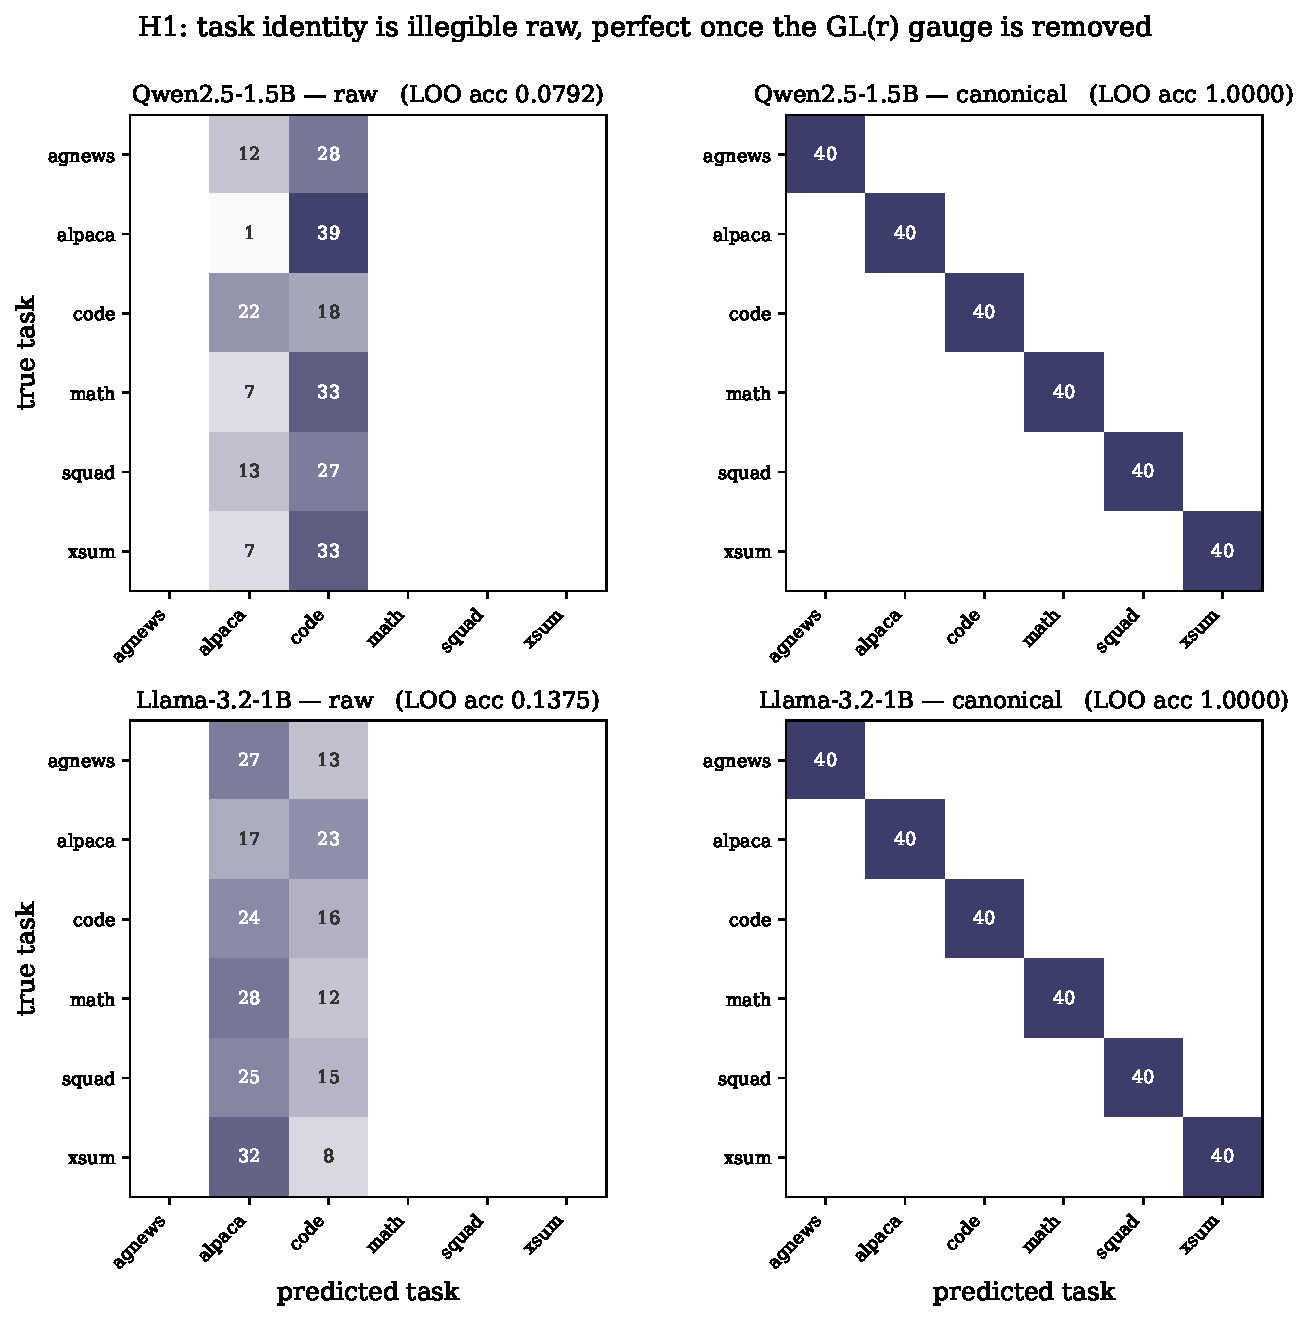
\includegraphics[width=0.95\textwidth]{figures-asset1/F1-h1-confusion.pdf}
\caption{H1 confusion matrices, raw vs canonical, per family: $6 \times 6$
heatmaps (rows true, columns predicted) showing raw scatter against the
canonical diagonal.}
\label{fig:f1}
\end{figure}

\paragraph{Raw carries weak signal, and the lock rejects it by design.}
Raw's tiny permutation $p$ alongside sub-threshold accuracy is not a
contradiction: raw weights carry a \emph{weak} recoverable signal
(per-class recall of 0.45 on code for Qwen, with every other class
$\le 0.025$; recall of 0.425 on alpaca plus 0.40 on code for Llama, with
every other class at 0) but come
nowhere near the 1.5$\times$ bar. This is exactly the case the two-sided
lock was built to reject---a representation that is statistically
distinguishable from noise but not usefully legible. We report the failure
as a failure.

\paragraph{Heterogeneity guard.} A perfect accuracy invites the suspicion
that the classifier is reading per-task variance scale rather than task
structure. The pre-registered variance-heterogeneity guard (Euclidean, in
the exact feature space the classifier saw) reads ratios of 1.00--1.46
across cells against a trigger of 3.7---not triggered. The canonical ceiling
is not a variance artifact.

\paragraph{Independent re-derivation.} The Director re-derived all eight LOO
accuracies from the per-family confusion matrices, then re-ran the canonical
LOO-SVM from scratch on the 88,704- and 50,688-dimensional feature matrices
(precomputed-Gram LOO, $C = 1.0$), obtaining 1.0000 for both families. The
ceiling result is real, not a summary artifact.

The reading: task identity lives in the adapter weights, but only becomes
\emph{legible} once the $\mathrm{GL}(r)$ gauge is removed. The
vocab-signature arm matches canonical at ceiling in both kv modes, so the
result is not specific to one canonicalization route. Within a controlled
family at coarse label granularity---6 tasks here, against the
up-to-312-class fine-grained label spaces of the W2T setting
(Section~\ref{sec:rw})---a linear probe suffices once the gauge is gone;
canonicalization, not classifier capacity, is the binding constraint.

\subsection{H2: the pre-registered prediction, refuted by its own control}
\label{sec:h2}

H2 was our boldest pre-registered prediction, and it was wrong. We predicted
that task structure would \emph{not} transfer across model families. The
verdict is \textbf{NOT supported}---and the refutation was produced by our
own triviality control, added in round-1 review before any data existed. We
regard this as the pre-registration working as designed, and we tell it in
that order.

\paragraph{The pinned decision rule.} Two dimension-agnostic representations
carry the analysis---spectrum (primary) and probe (corroborating), defined
in \S\ref{sec:d1}, with any disagreement between them reportable. The rule,
pinned by the Director on 2026-07-06 before the bank completed
(\S\ref{sec:prereg}): H2 (transfer fails) is supported iff, for BOTH
directions in the shift-controlled representation, (i) cross-family accuracy
is not significantly above chance at one-sided exact-binomial
$\alpha = 0.01$, and (ii) within-family accuracy exceeds cross-family
accuracy by $\ge 15$ percentage points. The shift-controlled variant is the
headline; raw transfer is descriptive. The constants
(\texttt{H2\_ALPHA = 0.01}, \texttt{H2\_MARGIN\_PP = 15.0}) are recorded in
the output JSON.

\paragraph{The triviality control.} The round-1 review fix required a
family-identity probe: before reading any transfer number, ask whether a
classifier can tell \emph{which family} an adapter came from.

\begin{table}[ht]
\centering
\caption{The triviality control. Raw representations perfectly encode
family identity; per-family standardization removes the family-mean
separation the raw probe exploited (standardized accuracies fall far below
chance---see text for why below-chance is the expected artifact, not
removal to chance).}
\label{tab:trivial}
\begin{tabular}{llcc}
\toprule
representation & variant & family-identity probe acc & chance \\
\midrule
spectrum & raw & 1.0000 & 0.5000 \\
spectrum & \texttt{family\_standardized} & 0.1521 & 0.5000 \\
probe & raw & 1.0000 & 0.5000 \\
probe & \texttt{family\_standardized} & 0.0000 & 0.5000 \\
\bottomrule
\end{tabular}
\end{table}

Raw representations encode the family perfectly (1.0000 against chance
0.5000; Table~\ref{tab:trivial}). A classifier trained on one family and
tested on the other is therefore tested under total covariate shift---raw
``transfer-at-chance'' would confirm our prediction while measuring nothing
but family scale. Per-family z-standardization
(\texttt{familywise\_standardize}) collapses the probe to 0.1521 (spectrum)
and 0.0000 (probe). Both standardized values sit far \emph{below} binary
chance 0.5---0.0000 means every cross-validated prediction is wrong---which
is the signature of standardizing on the full pool before cross-validation:
each held-out point is anti-correlated with its own family's fold mean, so
family membership remains decodable by inverting the probe. What the
control establishes is not that family information is annihilated but that
the family-\emph{mean} separation the raw probe exploited is gone; the
transfer verdict rests on the binomial tests of the transfer accuracies
themselves, not on the probe reading chance. The Director confirmed in
source that the
standardization is unsupervised---per-family z-scoring in which task labels
are never touched---so it removes family scale without any capacity to
manufacture task structure.

\paragraph{Transfer.} With the artifact removed, the picture inverts
(Table~\ref{tab:transfer}, Figure~\ref{fig:f2}):

\begin{table}[ht]
\centering
\caption{Cross-family transfer accuracy, raw vs family-standardized. Chance
$= 0.1667$. The headline is the standardized column, per the pinned rule;
raw is descriptive.}
\label{tab:transfer}
\begin{tabular}{llcccc}
\toprule
representation & direction & raw & standardized & binom $p$ (std) & margin \\
\midrule
spectrum & qwen$\rightarrow$llama & 0.1667 & \textbf{0.7833} & $7.70\times10^{-98}$ & 21.67pp \\
spectrum & llama$\rightarrow$qwen & 0.1667 & \textbf{0.7375} & $1.20\times10^{-84}$ & 26.25pp \\
probe & qwen$\rightarrow$llama & 0.1750 & \textbf{0.7792} & $1.37\times10^{-96}$ & 22.08pp \\
probe & llama$\rightarrow$qwen & 0.2167 & \textbf{0.7792} & $1.37\times10^{-96}$ & 22.08pp \\
\bottomrule
\end{tabular}
\end{table}

\begin{figure}[htbp]
\centering
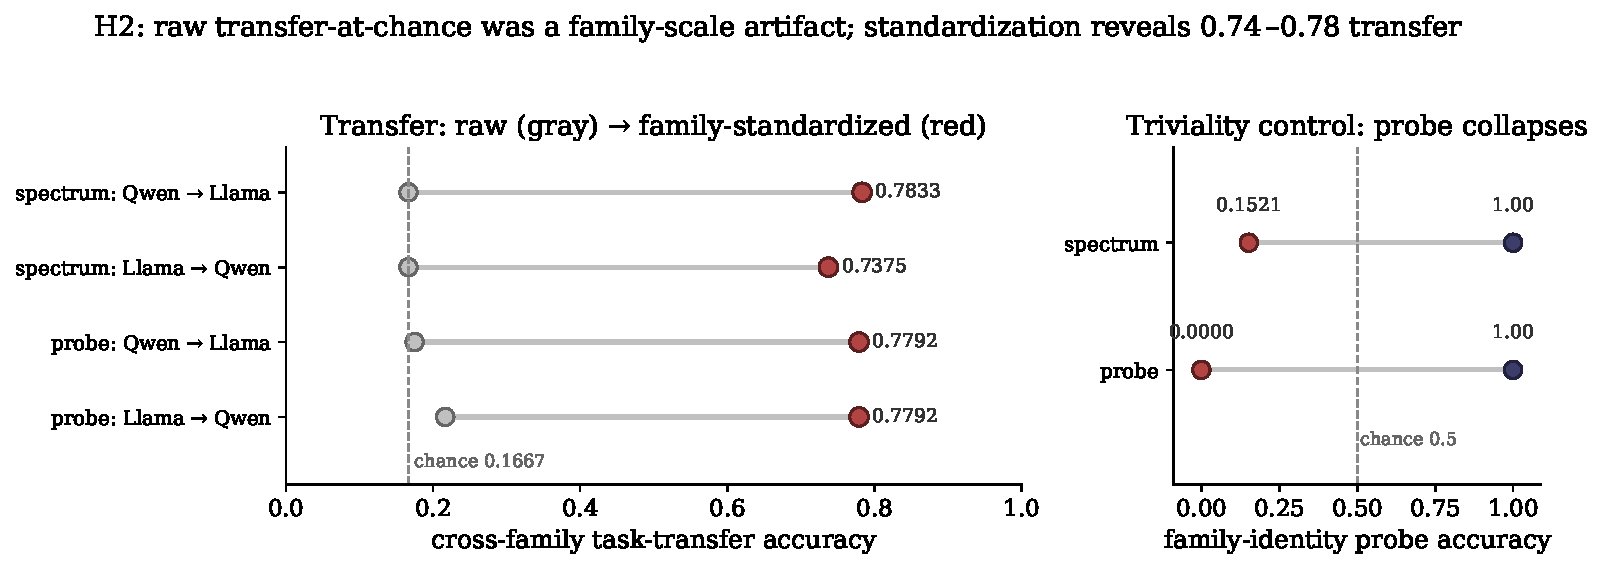
\includegraphics[width=0.85\textwidth]{figures-asset1/F2-h2-transfer.pdf}
\caption{H2 cross-family transfer: raw vs family-standardized accuracy per
direction and representation, with the chance line at 0.1667.}
\label{fig:f2}
\end{figure}

Raw transfer sits at or near chance in every direction---the number that
would have ``confirmed'' the prediction. Standardized transfer runs
0.7375--0.7833 across a 1.5B and a 1B model of different lineages, with
binomial $p$ between $7.70\times10^{-98}$ and $1.20\times10^{-84}$.
Condition (i) of the pinned rule fails decisively in both directions, in
both representations; spectrum and probe agree. One caveat on the $p$
magnitudes: the exact-binomial test treats the 240 test predictions per
direction as independent, but they cluster by task (6 task clusters
$\times$ 40 same-task adapters, with all-or-nothing per-class behavior), so
the effective sample size is smaller and the $p$-values are
anti-conservative as printed. The verdict does not lean on the exponents:
accuracies of 0.74--0.78 against chance 0.1667 clear $\alpha = 0.01$ under
any clustering-robust reading, and the $\ge 15$pp margin condition fails
independently of the test.

\paragraph{Verdict: H2 NOT supported.} The pre-registered ``transfer fails''
prediction is refuted. In the shift-controlled representation, task
structure transfers cross-family at ${\sim}74$--78\%. The finding is the
opposite of what we predicted, and the control added in review is exactly
what prevented a false confirmation on a covariate-shift artifact.

\paragraph{Independent re-derivation.} Because a pre-registration that flips
via a control added in review carries the highest motivated-reasoning risk
in the set, the Director re-ran the entire H2 pipeline end-to-end from the
spectrum and probe feature matrices, applying the standardization
independently. The triviality control reproduces (1.0000 raw $\rightarrow$
0.1521 / 0.0000 standardized); all four standardized transfer accuracies,
all four raw baselines, and all four binomial $p$-values reproduce to the
digit.

Had we run H2 without the triviality control, we would now be reporting a
confirmed prediction that is actually a measurement of family scale. The
cost of the control was one additional probe and a standardization pass; the
benefit was the difference between a false confirmation and a true
refutation. That asymmetry, not the transfer number itself, is what this
subsection is evidence for.

% ===================================================================
\section{Results II: Swap, merge, and gap}
\label{sec:results2}

\subsection{D2: the identity backbone is the sole load-bearing structure}
\label{sec:d2res}

\paragraph{Design.} D2 asks what a trained bridge is worth at inference
time, via the seven swap kinds defined in \S\ref{sec:d2}: cross-seed and
cross-task bridge swaps; the magnitude and topology components of the
cross-task swap (run unconditionally by Director override, not gated on any
data-dependent trigger); the identity bridge (the total contribution of
bridge training); and the two permutation cells that carry the structural
contrast---\texttt{permuted\_deviation} ($I + \mathrm{permute}(B - I)$, the
pinned H3 reference, which preserves the identity backbone) and the
full-entry \texttt{permuted} cell (a shared derangement of all 36 entry
positions, which destroys it). Both permutation cells share the same
derangement per (family, task, slot), so their difference isolates the
backbone effect and nothing else. $K = 3$ donor/recipient pairs per cell
gives 360 evaluations per family, every one re-assembled from the bank and
SHA-verified against the plan before evaluation, against the native adapter
on the recipient task's fixed 500-example split.

\paragraph{Result.} Table~\ref{tab:d2} gives the mean val-loss penalty
(evaluated minus native) by swap kind.

\begin{table}[ht]
\centering
\caption{D2 penalty matrix (mean val-loss penalty vs native, nats; 360
evals/family, of which 18 are native references; penalty cells have
$n = 90$ for the cross-task, magnitude, and topology kinds and $n = 18$
elsewhere. The
\texttt{permuted} means carry per-eval spread: SD 2.31 (qwen) and 3.34
(llama) at $n = 18$.)}
\label{tab:d2}
\begin{tabular}{lcc}
\toprule
swap kind & \texttt{qwen2.5-1.5b} & \texttt{llama3.2-1b} \\
\midrule
\texttt{cross\_seed} & $+0.0000$ & $+0.0002$ \\
\texttt{cross\_task} & $+0.0000$ & $+0.0003$ \\
\texttt{cross\_task\_magnitude} & $+0.0000$ & $+0.0000$ \\
\texttt{cross\_task\_topology} & $+0.0000$ & $+0.0002$ \\
\texttt{identity} & $+0.0000$ & $+0.0007$ \\
\texttt{permuted\_deviation} (H3 reference) & $+0.0000$ & $+0.0007$ \\
\textbf{\texttt{permuted} (full)} & $\mathbf{+2.8086}$ & $\mathbf{+3.8365}$ \\
\bottomrule
\end{tabular}
\end{table}

\begin{figure}[htbp]
\centering
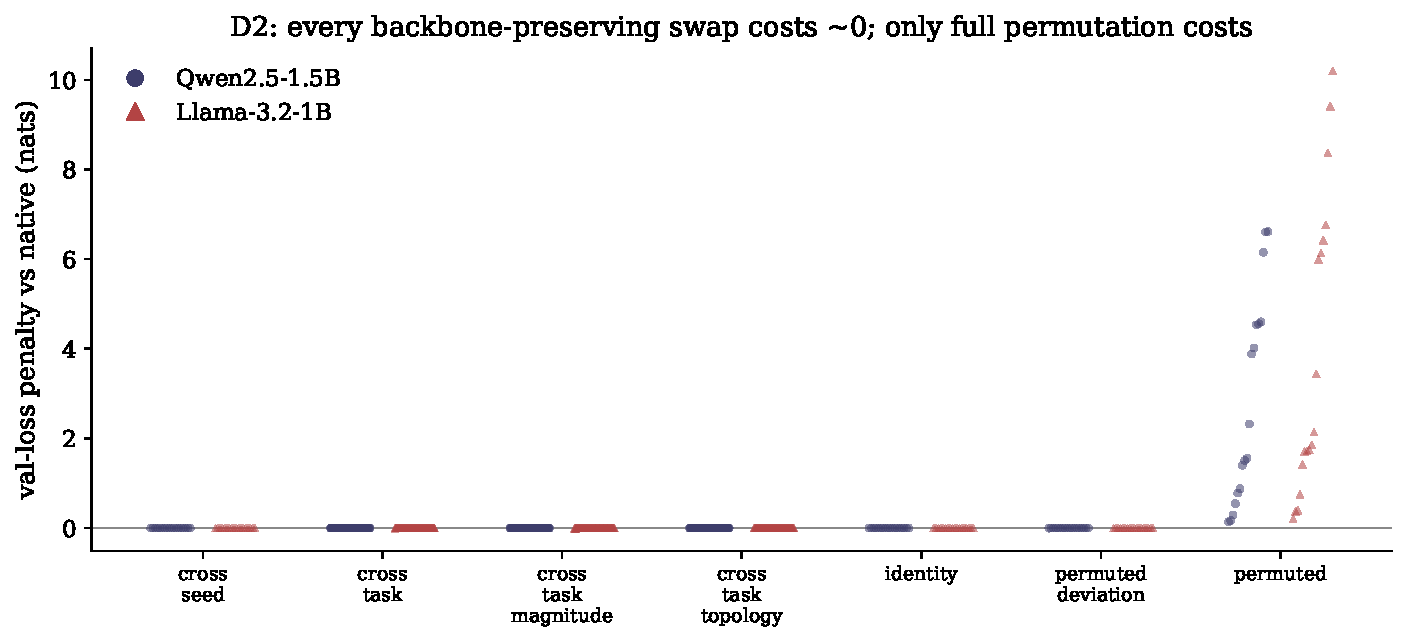
\includegraphics[width=0.85\textwidth]{figures-asset1/F3-d2-penalties.pdf}
\caption{D2 per-eval val-loss penalties by swap kind: the ${\sim}0$ cluster
against the $+2.8$/$+3.8$ full-entry permutation.}
\label{fig:f3}
\end{figure}

Installing a different task's trained bridge into an adapter costs
essentially nothing. So does deleting the trained bridge entirely
(\texttt{identity}), and so does scrambling the trained deviation while
preserving the backbone (\texttt{permuted\_deviation}). Only the full-entry
permutation---the one operation that destroys the identity backbone---costs
anything, and it costs 2.8 to 3.8 nats. The contrast between the two
permutation cells, which differ only in whether the backbone survives,
isolates the backbone as the sole load-bearing structure for
in-distribution loss. This is the H3 verdict: the \emph{substrate}
hypothesis is supported---cross-task penalties sit at the cross-seed
baseline ($+0.0000$/$+0.0003$ vs $+0.0000$/$+0.0002$)---and the
task-specific hypothesis is refuted; the cross-task penalty is neither
large nor does it scale with between-task distance (the magnitude and
topology decomposition cells are both ${\sim}0$). This is consistent with the bank's controller-free,
identity-init design, and it sharpens the reading of D-aux below: the
trained bridge deviation is real and measurable, but it is not what the loss
depends on.

The Director's regrade reproduced all 14 per-kind means exactly from the 360
per-eval rows per family.

\paragraph{Cost.} D2 is the pipeline's first GPU commitment: 360 val-loss
evaluations per family, each requiring assembly, SHA verification, and a
full pass over the recipient's 500-example split. The decomposition cells
alone add 180 evaluations per family---the price of running the guard
unconditionally rather than gating it on whether a contradiction
materialized.

\subsection{D3: post-hoc, weight-only merge-conflict prediction}
\label{sec:d3res}

\paragraph{Scope.} arXiv:2606.19549 \citep{mergeprobe2026} owns the
training-time form of merge-conflict prediction (Section~\ref{sec:rw}). D3
is the weight-only, post-hoc regime---two finished adapters, no training
access, no activations, no data---and we claim only this regime.

\paragraph{Design and dated amendment.} $N = 120$ vertex-disjoint pairs per
family (each run used at most once---the dyadic-dependence-safe design),
$\alpha = 0.5$ midpoint merges. The pair design was pre-declared with
per-cell task-pair stratification and amended, the same day and before any
pair, merge, or label existed, to the uniform vertex-disjoint sampler the
frozen tool actually implements; \S\ref{sec:d3design} gives the full
timeline and the Director's ruling (``clean dated amendment (L-006 / R10);
no objection''). The realized (task$_i$, task$_j$) cell coverage is reported
descriptively (Figure~\ref{fig:f5}): against an expected ${\sim}16\%$
same-task under uniformity (${\sim}20$/120 pairs), the realized same-task
counts are 14/120 (11.7\%) for qwen and 22/120 (18.3\%) for llama.

\begin{figure}[htbp]
\centering
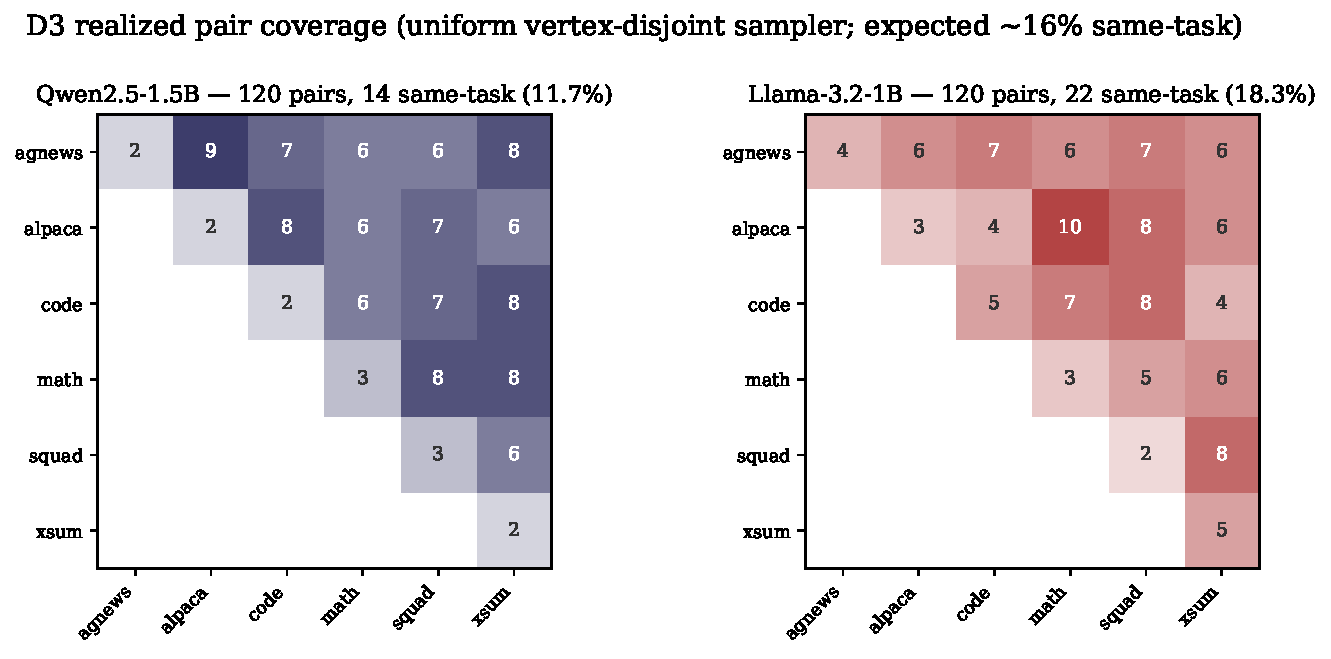
\includegraphics[width=0.85\textwidth]{figures-asset1/F5-d3-coverage.pdf}
\caption{D3 realized (task$_i$, task$_j$) pair-cell coverage under the
uniform vertex-disjoint sampler (amendment transparency): same-task fraction
realized 14/120 (qwen) and 22/120 (llama) against the ${\sim}16\%$
same-task expected under the amended uniform declaration.}
\label{fig:f5}
\end{figure}

\paragraph{Labels.} The primary label rule was pinned by the Director before
the bank completed: a pair is a conflict if the merge degrades either
endpoint task by $\ge 5\%$ relative to that endpoint's native adapter, with
a degenerate floor of 10\% triggering fallback to the pre-declared median
split. The rule held: the pooled conflict rate is 85.8\%
(\texttt{frac\_positive}
0.8583, identical at both endpoints), above the floor, so the primary rule
stands and no fallback was used. Per family: qwen 99 conflicts / 21
non-conflicts (82.5\%), llama 107 / 13 (89.2\%)---llama's minority fraction
(10.8\%) clears the 10\% floor by a single pair, so the llama AUC and its
CI rest on 13 negative pairs (a limitation reported in
Section~\ref{sec:limitations}). A conflict rate this high is itself a
finding about midpoint merging in this bank: at $\alpha = 0.5$, most pairs
degrade at least one endpoint by 5\% in relative perplexity. Native
reference values derive from the
trainer's recorded final val losses (exponentiated to perplexity), after
verifying 0.00000\% divergence against 36
fresh D2-harness evaluations.

\paragraph{Features and model.} The feature sets and classifier are fixed in
\S\ref{sec:d3}: a 2-feature \texttt{distance} baseline
(\texttt{cos\_distance}, \texttt{l2\_distance}) against the \texttt{full}
weight-only set (those two, the four gauge-invariant principal-angle
aggregates, and the per-module \texttt{module\_l2} and
\texttt{module\_angle\_mean} vectors), under logistic regression, 5-fold CV
with fold seed 0, and 1000 bootstrap resamples---all pinned in the report
JSON.

\paragraph{Result.} Table~\ref{tab:d3} gives the headline group-aware AUCs.

\begin{table}[ht]
\centering
\caption{D3 merge-conflict prediction, group-aware CV AUC with 95\%
bootstrap CIs (120 pairs/family; pooled OOF row descriptive).}
\label{tab:d3}
\small
\begin{tabular}{lccc}
\toprule
family & AUC full (weight-only) & AUC distance-only & full $-$ distance \\
\midrule
\texttt{qwen2.5-1.5b} & \textbf{0.995} [0.983, 1.000] & 0.675 [0.484, 0.848] & $+0.320$ [0.150, 0.511] \\
\texttt{llama3.2-1b} & \textbf{0.962} [0.898, 0.999] & 0.713 [0.458, 0.923] & $+0.249$ [0.039, 0.490] \\
pooled OOF (descriptive) & 0.9890 [0.9730, 0.9992] & 0.7082 & $+0.2808$ [0.1565, 0.4205] \\
\bottomrule
\end{tabular}
\end{table}

\begin{figure}[htbp]
\centering
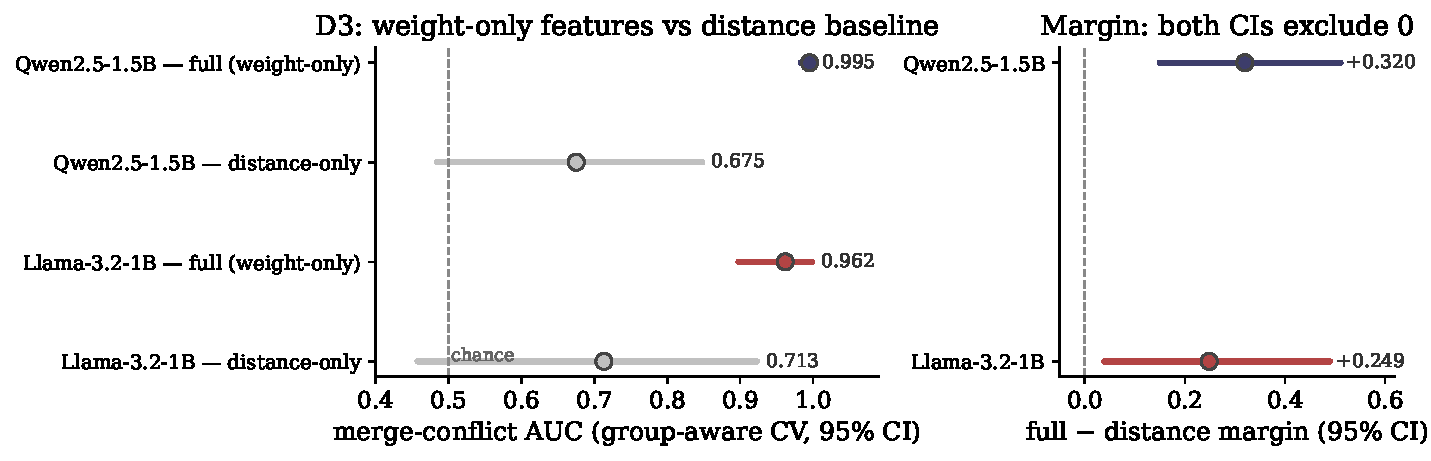
\includegraphics[width=0.85\textwidth]{figures-asset1/F4-d3-auc.pdf}
\caption{D3 merge-conflict AUC, full vs distance-only feature sets, per
family: point estimates with 95\% group-aware bootstrap CIs against the
chance line (left) and the full-minus-distance margin CIs (right).}
\label{fig:f4}
\end{figure}

Two adapters' weights alone predict whether their midpoint merge degrades an
endpoint, at AUC 0.96--0.99, and the gauge-invariant block adds a margin
over raw distance whose CI excludes zero in both families. The headline is
group-aware CV (StratifiedGroupKFold over run-overlap components with a
component-cluster bootstrap); because the vertex-disjoint design produced
120 single-pair components per family, there is no dyadic dependence to
correct, and group-aware and naive numbers agree to within CV-fold reshuffle
noise (llama full 0.962 group-aware vs 0.952 naive; qwen 0.995 under both).

\paragraph{The distance-only baseline is fold-scheme-sensitive.} The same
naive-vs-group-aware split visible in the full model above is larger for the
baseline: the Director's independent from-scratch re-run, which used a plain
StratifiedKFold (the naive scheme), reproduced the report's naive block
exactly---distance 0.686 (qwen) / 0.667 (llama), full 0.995 / 0.952---
against the group-aware headline's 0.675 / 0.713. The ${\sim}0.01$--0.05
gap is fold-scheme variance on a 2-feature model over 120 points, not seed
noise. The full-model result and the existence of the margin are not in
question, but the lower end of the margin-over-distance CI depends on this
baseline, which is why the fold configuration (scheme, seed $= 0$,
n\_splits $= 5$) is pinned and the fragility reported rather than averaged
away.

\paragraph{Interpretive caveats.} Invertible bridges are a gauge on the
update column space, so the principal-angle features are provably
insensitive to bridge numerics; whatever bridge information reaches the
classifier arrives through the magnitude weights and the raw distances. The
margin over distance is therefore evidence about update geometry, not about
the bridge---consistent with D2's finding that the bridge carries no
in-distribution loss structure. A second caveat binds the margin itself:
the conflict label is strongly associated with task composition (same-task
pairs are predominantly non-conflict for qwen---13 of 14---and negatives
are dominated by same-task pairs: 13 of 21 for qwen, 9 of 13 for llama),
and H1 established that task identity is fully recoverable from weight
features. A task-composition oracle alone (score 1 iff cross-task) reaches
AUC 0.804 (qwen) / 0.785 (llama)---already above the distance-only
baseline---so part of the margin over distance rides on task
identification. The full model exceeds the oracle bound (0.995 / 0.962),
so geometric signal beyond task identity is present, but the
discriminative value \emph{within} the cross-task-only regime is smaller
than the headline AUC and was not separately pre-registered; we bound it
rather than claim it (Section~\ref{sec:limitations}).

\paragraph{Cost.} D3's labels required GPU evaluation of 240 merged adapters
on both endpoint tasks' val splits, on top of the CPU feature extraction.
The labels runner had no shipped implementation (the analysis-pipeline
documentation scoped it
``external''); it was written post-card and put through a fresh-context
adversarial verification before its GPU run, which caught two blocking
defects (a flat-vs-nested merge-loading bug and a machine-absolute manifest
path)---both fixed and dry-run-verified before launch.

\subsection{D-aux: the pilot correlation shrinks honestly}
\label{sec:dauxres}

\paragraph{Design.} D-aux re-verifies the pilot's headline
association---bridge deviation predicts generalization gap---at bank scale,
as the Director's pinned condition for including it at all (``Re-verify
$r = 0.888$ \ldots\ on the bank''). The primary pre-registered pair is
\texttt{dev\_mean} (mean over modules of
$\lVert \mathrm{bridge}_{\mathrm{final}} - I \rVert_F$) against
\texttt{final\_gap} (val minus train at step 2000), $n = 480$. The step-0
identity control comes out 0.0 exactly, as it must by construction.
Within-task cells are the pre-registered Simpson's-paradox guard:
descriptive, but shown, not hidden.

\paragraph{Result.} Table~\ref{tab:daux} gives the pooled claim and the
guard cells.

\begin{table}[ht]
\centering
\caption{D-aux bridge-deviation $\leftrightarrow$ generalization-gap
correlation (Pearson $r$, 95\% bootstrap CIs).}
\label{tab:daux}
\begin{tabular}{lccc}
\toprule
cell & $n$ & Pearson $r$ & 95\% CI \\
\midrule
pooled & 480 & 0.300 & [0.175, 0.415] \\
\texttt{qwen2.5-1.5b} & 240 & 0.418 & [0.323, 0.522] \\
\texttt{llama3.2-1b} & 240 & 0.337 & [0.201, 0.466] \\
within math (llama) & 40 & 0.549 & [0.324, 0.736] \\
within math (qwen) & 40 & 0.336 & [0.030, 0.652] \\
within xsum (qwen) & 40 & $-0.301$ & $[-0.502, -0.066]$ \\
\bottomrule
\end{tabular}
\end{table}

\begin{figure}[htbp]
\centering
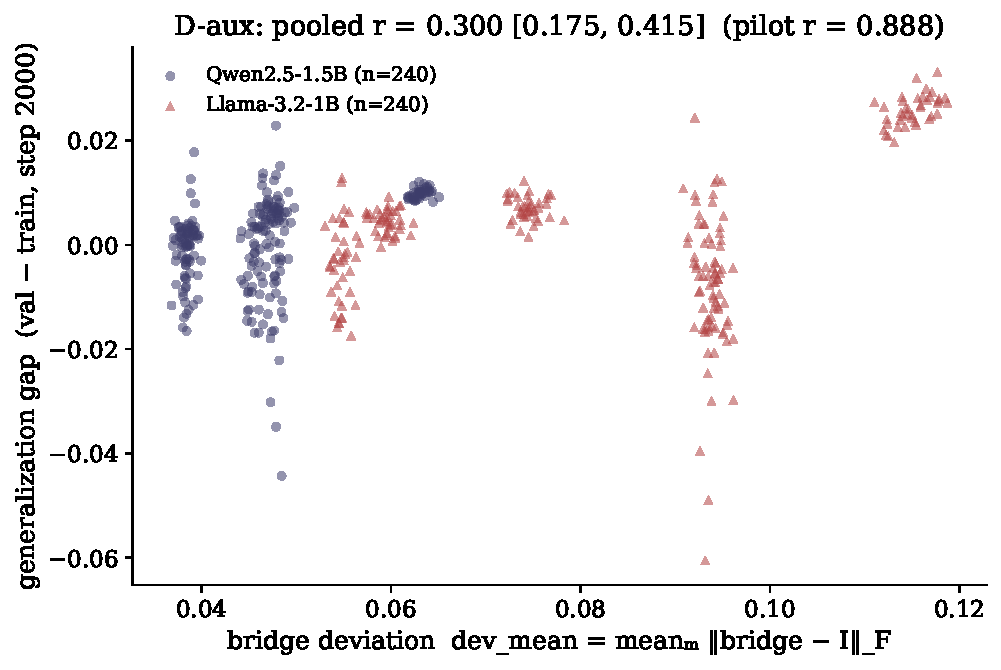
\includegraphics[width=0.85\textwidth]{figures-asset1/F6-daux-scatter.pdf}
\caption{D-aux scatter: \texttt{dev\_mean} vs \texttt{final\_gap}, 480
points, colored by family; pooled $r$ annotated.}
\label{fig:f6}
\end{figure}

\begin{figure}[htbp]
\centering
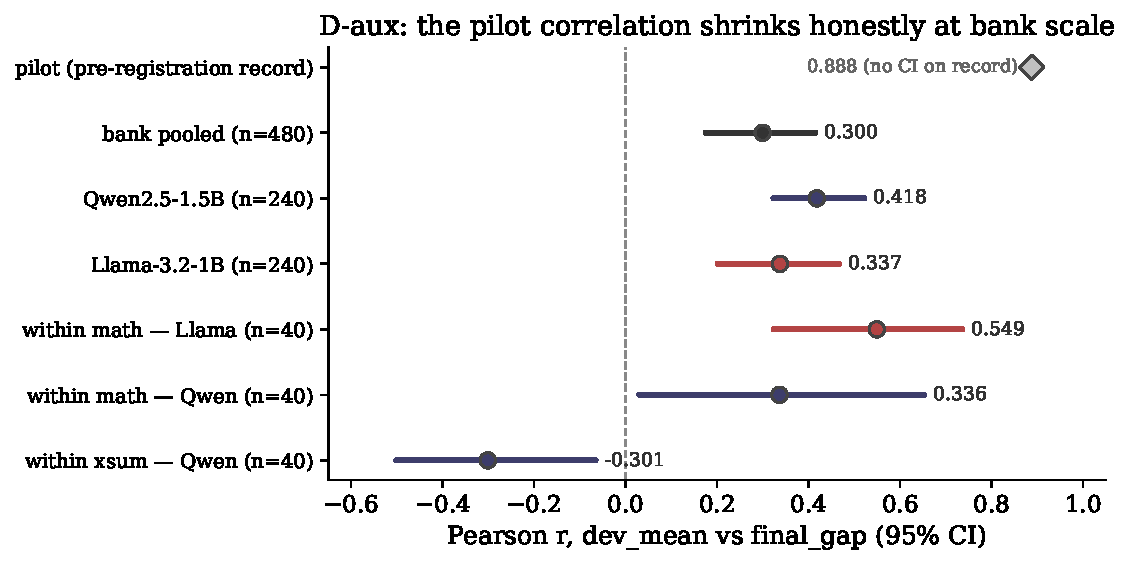
\includegraphics[width=0.85\textwidth]{figures-asset1/F7-daux-forest.pdf}
\caption{The D-aux shrink: pilot $r = 0.888$ against the bank pooled and
per-cell correlations (forest plot).}
\label{fig:f7}
\end{figure}

The pilot's $r = 0.888$ does not survive the bank, and we report that as the
result. Pooled over 480 runs the association is real, positive, and
non-zero---$r = 0.300$ [0.175, 0.415]---but modest, and inflated in the
pilot by small-$n$ and task mixture. Within task it is heterogeneous: math
is positive in both families (0.549 llama, 0.336 qwen), while xsum in qwen
is significantly negative ($-0.301$ $[-0.502, -0.066]$). The pooled
bank-level correlation remains the claim; the cells bound what it can mean.
A deviation measure whose within-task sign flips between cells is not a
universal overfitting signal---it is a between-task association with real
but task-dependent within-task structure.

The 0.888 $\rightarrow$ 0.300 shrink is a success of the protocol, not a
failure of the result. The pilot number was computed on a small mixed
sample; the pre-registered re-verification on 480 runs is exactly the check
that separates a real-but-modest association from an artifact of the sample
that first suggested it. The Director's regrade reproduced the pooled and
per-family values from the 480 (\texttt{dev\_mean}, \texttt{final\_gap})
pairs.

\paragraph{Reading D2 and D-aux together.} D-aux shows the trained bridge
deviation carries real signal about training dynamics---it correlates with
the generalization gap. D2 shows that same deviation is worth ${\sim}0$ nats
to in-distribution loss, and that only the identity backbone is
load-bearing. Both are true, and their conjunction is the finding: the
bridge records where the run has been without determining where the loss
sits. D-aux is CPU-only and rides along at negligible cost; its price was
paid once, in the pilot's discipline of flagging its own $n$.

% ===================================================================
\section{Discussion}
\label{sec:discussion}

\paragraph{The gauge, not the information, was the obstacle.} The two
identifiability results share one mechanism. In H1, raw adapter weights fail the
task-identity lock (LOO accuracy 0.0792 qwen / 0.1375 llama against the
1.5$\times$-chance bar of 0.2500, chance 0.1667), while the
$\mathrm{GL}(r)$-canonical representation identifies all six tasks at 1.0000
in both families---at a fraction of the dimensionality (88,704 / 50,688
features against 6,541,248 / 5,114,112 raw). The task signal was in the
weights the whole time; raw's tiny permutation $p$ (0.000999) with
sub-threshold accuracy shows a weak recoverable trace (code recall 0.45 for
qwen; alpaca 0.425 and code 0.40 for llama), but the factorization gauge
buries it below the lock. In H2,
the same story repeats one level up: raw cross-family transfer sat at
chance, and the triviality control revealed why---a linear probe reads
family identity from raw features at 1.0000, so raw ``transfer failure'' was
family-scale covariate shift, not absent structure. Unsupervised per-family
standardization collapses the family probe to 0.1521 (spectrum) / 0.0000
(probe projection) and transfer rises to 0.7375--0.7833 (binomial
$p \le 1.20\times10^{-84}$). One reading covers both: nuisance
variation---the $\mathrm{GL}(r)$ factorization gauge within a family, the
scale gauge between families---dominates raw weight coordinates and obscures
task structure that is intact underneath. Task identity is gauge-obscured,
not absent. The scope of this claim runs on the label-granularity axis: our
six coarse tasks are the opposite regime from W2T's fine-grained attribute
label spaces (312 binary attributes over 10k+-adapter collections), and we
make
no claim about what a linear probe recovers, raw or canonical, at that
granularity.

\paragraph{The backbone is load-bearing; the trained bridge deviation is
real but cheap.} D2 and D-aux look contradictory until they are read
together. D-aux shows the trained bridge deviation is a real, measurable
quantity: it correlates with the generalization gap at $r = 0.300$
[0.175, 0.415] pooled over all 480 runs, with the step-0 identity control at
0.0 exactly. D2 shows the same deviation is nearly worthless to
in-distribution loss: installing a different task's trained bridge costs
$+0.0000$ (qwen) / $+0.0003$ (llama) nats of val loss, and even permuting
the trained deviation while keeping the identity backbone
(\texttt{permuted\_deviation}, the pinned H3 reference) costs $+0.0000$ /
$+0.0007$. Only the full-entry permutation, which destroys the identity
backbone itself, costs anything: $+2.8086$ / $+3.8365$ nats. The resolution
is that the deviation carries information \emph{about} the run---enough for
a weak correlate of its generalization gap---without carrying the
in-distribution task solution, which lives in the identity backbone the
controller-free, identity-init design builds in. The bridge is a
diagnostic-bearing structure, not a load-bearing one.

\paragraph{Angles predict merge conflict, post-hoc, from weights alone.} D3
closes the loop from description to prediction: two adapters' weights, with
no training access and no evaluation of the merge, predict whether their
$\alpha = 0.5$ midpoint merge degrades either endpoint by $\ge$5\%
relative, at group-aware AUC 0.995 [0.983, 1.000] (qwen) / 0.962
[0.898, 0.999] (llama). The margin over a distance-only baseline ($+0.320$
[0.150, 0.511] / $+0.249$ [0.039, 0.490], both CIs excluding 0) is what
makes this a geometry result rather than a magnitude result: the
gauge-invariant principal-angle block is what raw cosine and L2 distance
lack. One interpretive caveat is pinned in the pipeline: invertible bridges
are a gauge on the update column space, so principal-angle features are
provably insensitive to bridge numerics---bridge information reaches the
classifier only through the magnitude weights and raw distances. The scope
boundary is equally pinned: arXiv:2606.19549 \citep{mergeprobe2026} owns the
training-time form of merge-conflict prediction; this result is weight-only
and post-hoc, and we claim only that regime.

\paragraph{What pre-registration bought.} Two of the five results went
against us, and those two are the credibility of the other three. The H2
prediction---that task structure would not transfer across families---was
refuted, and refuted specifically by the triviality control added in round-1
review: without the family-identity probe, raw transfer-at-chance would have
read as a confirmation, and it would have been false. A pre-registration
that flips via its own control is the protocol working as designed, not
failing. The D-aux pilot correlation shrank from $r = 0.888$ to $r = 0.300$
[0.175, 0.415] at bank scale---small-$n$ and task-mixture inflation, exposed
by the pre-declared Simpson's-guard cells, which also show the association
is heterogeneous within task (llama math 0.549 [0.324, 0.736]; qwen xsum
$-0.301$ $[-0.502, -0.066]$). A pipeline that can only confirm is not
measuring; this one refuted its boldest prediction and deflated its own
pilot, under an interlock that made post-hoc rescue impossible.

\paragraph{Run-log honesty.} Three operational facts belong in the record
rather than a drawer. D1's first launch died on a default-HF-cache
environment trap; it was environment-level, nothing was unblinded, and the
relaunch was clean. The D3 label generator had no shipped runner (the
analysis-pipeline documentation scoped it ``external''); the runner written
for it was put
through a fresh-context adversarial verification \emph{before} its GPU run,
which caught two blocking defects (a flat-vs-nested merge-state loader bug
and a machine-absolute manifest path), both fixed and dry-run-verified
before launch. And the native-loss shortcut---taking natives from the
trainer's metrics rather than re-evaluating---was verified at 0.00000\%
divergence against 36 fresh D2 harness evaluations before use. Maker--grader
separation was applied exactly where the pipeline was newest.

\subsection{Limitations}
\label{sec:limitations}

Cost first: the bank consumed roughly 17 days of a single local GPU
(2026-07-03 to 2026-07-20, including the A1 geometry restart), with four
HF-Hub-504 failures retried to completion. The analyses themselves are
cheap---D1, D-aux, and D3 feature extraction are CPU-only---but the artifact
they require is not.

\paragraph{Two families at ${\sim}1$--1.5B scale.} The bank spans
Qwen2.5-1.5B-Instruct and Llama-3.2-1B-Instruct: two lineages, but both
small instruct-tuned decoders. The H2 transfer result crosses these two
families and no others; whether canonicalization ceilings, backbone
dominance, or angle-based merge prediction hold at 7B+ scale or across
architecture classes is unmeasured.

\paragraph{Six coarse tasks.} The label-granularity axis cuts both ways. Our
regime---6 coarse task labels, 40 seeds each---is where a linear probe on
canonical features reaches ceiling; we make no claim about fine-grained
regimes such as W2T's 312-binary-attribute label space, in either
direction. Ceiling accuracy on six classes also means H1 cannot rank
representations above the lock: canonical and vocab-signature all sit at
1.0000, and separating them would need a harder label space.

\paragraph{In-distribution val loss only.} Every D2 penalty and every D3
label rests on loss over fixed 500-example validation splits
(\texttt{val\_seed} 777) of the training task's own distribution. The D2
conclusion is explicitly in-distribution: the bridge deviation is negligible
to \emph{this} loss. Behavioral, out-of-distribution, or
instruction-following consequences of bridge swaps and merges are
unmeasured, and D-aux's $r = 0.300$ against the generalization gap is a hint
that the deviation matters for something val loss on the training
distribution does not fully capture.

\paragraph{Single merge operator.} D3 predicts conflict for $\alpha = 0.5$
midpoint merges only. Other $\alpha$ values, TIES/DARE-style merge
operators \citep{yadav2023ties,yu2023dare}, and merges of more than two
adapters are outside the measured
claim.

\paragraph{Uniform pair sampling, by dated amendment.} The D3 pair design
was pre-declared with per-cell stratification
over task pairs, then amended---before any pairs, merges, or labels
existed (\S\ref{sec:d3design} gives the artifact-anchored timeline)---to
the uniform vertex-disjoint
sampler the frozen tool actually implements; the Director approved it as a
clean dated amendment (L-006 / R10).
The consequence is uneven realized coverage of the 21 task-pair cells
(expected ${\sim}16\%$ same-task under uniformity; realized 11.7\% qwen /
18.3\% llama), reported descriptively; per-cell conflict-rate estimates are
correspondingly noisy, and the headline AUC is a claim about the uniform
pair population, not any single cell.

\paragraph{D3 baseline fold-scheme sensitivity.} The cross-validation
configuration is pinned: group-aware StratifiedGroupKFold, fold seed 0, 5
splits, logistic model, 1,000 bootstrap resamples. The Director's
independent naive-CV re-run reproduced the report's naive block exactly
(distance 0.686 / 0.667, full 0.995 / 0.952); the group-aware headline reads
0.675 / 0.713 for the baseline---a fold-scheme difference of
${\sim}0.01$--0.05 on a 2-feature model over 120 points, not seed noise. The
full-model result and the existence of the margin are not in question, but
the lower end of the margin-over-distance CI depends on the baseline, which
is why the fold configuration is pinned and the fragility is reported rather
than averaged away.

\paragraph{D-aux heterogeneity.} The pooled $r = 0.300$ conceals
sign-varying within-task structure: math is positive in both families
(0.549 llama, 0.336 qwen) while xsum in qwen is significantly negative
($-0.301$ $[-0.502, -0.066]$). The pooled bank-level claim is the
pre-registered one; any within-task use of the deviation--gap association
would need task-specific calibration this bank is only pilot-scale for
($n = 40$ per cell).

\paragraph{One bridge architecture.} The bank's adapters carry the house
6-channel identity-initialized, controller-free bridge
(\S\ref{sec:bank})---not present in standard PEFT LoRA. D2's backbone
result and D-aux's deviation--gap association are properties of this
design; bridges trained under a controller or from non-identity
initialization could be load-bearing, and standard bridgeless LoRA is
outside the D2/D-aux measured claim. H1, H2, and D3 operate on the
effective update and are less exposed, but the bank itself is
single-architecture.

\paragraph{One training recipe.} Every adapter shares a single
hyperparameter configuration (rank 24, $\alpha$ 16, LR $2\times10^{-4}$,
2000 steps, one data budget; Table~\ref{tab:t1-bank-design}), varying only
family, task, and seed. Task identifiability, transfer, backbone dominance,
and merge-conflict prediction are all measured \emph{within} this recipe;
banks heterogeneous in rank, LR, or steps could couple recipe to task and
change every result. The canonical feature projection is likewise a single
pinned draw (\texttt{proj\_seed} 0); projection-seed sensitivity of the H1
ceiling is unmeasured.

\paragraph{Conflict label vs.\ task composition.} The D3 conflict label is
strongly associated with task-pair identity: same-task pairs are
predominantly non-conflict, and the negative class is dominated by
same-task pairs (13 of 21 qwen, 9 of 13 llama). Since H1 shows task
identity is fully recoverable from these features, a task-composition
oracle alone reaches AUC 0.804 / 0.785---above the distance baseline---so
the headline AUC upper-bounds the predictor's discriminative value within
the cross-task-only regime (\S\ref{sec:d3res}). A cross-task-only or
composition-controlled evaluation was not pre-registered and is future
work.

\paragraph{Small negative class.} At the realized conflict rates the
discriminative estimates rest on 21 (qwen) and 13 (llama) non-conflict
pairs; llama's minority fraction (10.8\%) clears the pre-registered 10\%
degenerate-balance floor by a single pair. The CIs reflect this (llama
margin lower bound 0.039), and any re-weighting of the label rule would
need a fresh pre-registration.

% ===================================================================
\section{Reproducibility}
\label{sec:repro}

Every headline number in this paper is re-derivable from a per-item
verification bundle, and every one has already been re-derived by someone
who was not us. The bundle (\path{results/asset1-delivery-verify/})
carries two tiers. Tier 1 is per-item result data: the per-family
$6\times6$ confusion matrices and permutation summaries behind every H1
accuracy; the full H2 transfer and family-identity-probe tables; 360
per-eval D2 rows per family, each with its assembly SHA-256 and val loss;
240 per-pair D3 feature dicts and labels with per-endpoint merged and native
perplexities; and 480 per-run D-aux (\texttt{dev\_mean},
\texttt{final\_gap}) rows. Tier 2 is the reduced feature matrices
(\texttt{features\_<family>.npz}, 90.6 MB qwen / 56.7 MB llama, float32),
exported by the frozen D1 feature functions so a from-scratch classifier
re-run bit-matches. Feature extraction and all Tier-1 outputs are
deterministic---fixed seeds, no wall-clock dependence---with recompute
recipes per analysis in the bundle README.

The bundle is anchored: rhombic commit \texttt{638f4a8}, archive SHA-256\\
{\small\texttt{c1891d50fc7c48c27d6fb606d667f1f1120105ed55cb7414c8e4b3d874acfadd}},\\
all 16 files matching the SHA256SUMS manifest
byte-for-byte. The independent Director regrade worked from exactly those
bytes and re-derived every headline: H1 accuracies reproduced from the
confusion matrices and the canonical LOO-SVM re-run from scratch on the
feature matrices (1.0000 both families); the entire H2 pipeline re-run
end-to-end from the spectrum and probe matrices, with the standardization
applied independently and \texttt{familywise\_standardize} confirmed
unsupervised in source; all 14 D2 per-kind means reproduced exactly from
per-eval rows; the D3 conflict rate (0.858) and full-model AUC reproduced
from raw labels and pairs; and the D-aux correlations reproduced from the
480 per-run pairs. The one deviation found---the D3 distance-baseline
fold-scheme sensitivity, initially misdiagnosed as seed noise and corrected
in the Director's re-versioned sign-off---is reported above as a limitation,
per the Director's write-up requirement.

Upstream of the bundle, the analysis layer itself is the reproducibility
mechanism. A completeness interlock (\texttt{require\_complete\_bank})
refused every real-bank statistic until the manifest showed 480/480
COMPLETE, so all five analyses ran against the finished bank exactly once,
with every open analytical choice pinned by the Director before completion
and recorded in each tool's output JSON; deviations are dated amendments in
the record, never silent revisions. The tooling passed 171/171 tests plus
the D1/D3/D-aux synthetic selftests, re-verified on delivery day before any
real-bank command ran.

Hardware and stack: the bank trained on a single NVIDIA RTX 6000 Ada
(48\,GB); every run's \texttt{config.json} records its library versions
(PyTorch, CUDA) alongside its seeds and cohort tags, so the software stack
is reconstructable per run rather than asserted here.

Release scope: the verification bundle (Tier 1) and all analysis code ship
in the public rhombic repository with this paper; the reduced feature
matrices (Tier 2, ${\sim}147$\,MB) are published on Hugging Face alongside
it. The adapter bank itself (480 trained runs) remains a local artifact
for size; its manifest, per-run configs, and the trainer that reproduces
it are in the repository.

% ===================================================================
\section*{Acknowledgments}
Experimentation, analysis, and drafting were performed with a standing AI
research collaborator (Claude, Anthropic). The Director role was performed
by a separate Claude instance with no shared context: it received artifacts
and returned dated rulings, pinning open analytical choices before the
consuming analyses ran, and it re-derived every headline quantity from
per-item data---H1 and H2 re-run from the feature matrices; the D3
from-scratch re-run under the naive fold scheme, with the group-aware
headline verified against the pinned report; three related-work citation
re-verifications taken on report and not independently checked. The
Director was isolated from the analysis process, not blinded to results;
its rulings and regrades are archived as dated documents in the
repository. All numbers reported here were machine-verified against the
frozen artifacts rather than restated from any model's summary.

% ===================================================================
% Figures note: Tables T2--T7 from the outline are realized in-text;
% figures F1--F7 are placed near their first reference. T1 (bank design)
% and the dataset table are AUTO-GENERATED by paper/make_t1.py from
% asset1_bank.py + asset1_datasets.py + bank_manifest.json.
% House palette rules: rhombic/CLAUDE.md; figure conventions follow
% paper/figures-asset1/make_figures.py.

% ===================================================================
% --- references ---
\bibliographystyle{plainnat}
\bibliography{refs-asset1}

\end{document}
